% Paquetes
\documentclass[a4paper,11pt]{article}
\usepackage[utf8]{inputenc}
\usepackage{graphicx}
\usepackage{hyperref}
\usepackage{geometry}
\usepackage{ragged2e}
\usepackage{setspace}
\usepackage{anyfontsize}
\usepackage{tocloft}
\usepackage{titlesec}
\usepackage{parskip}
\usepackage{indentfirst}
\usepackage{textcomp}
\usepackage[spanish]{babel}
\usepackage{caption}
\usepackage[square,numbers]{natbib}
\usepackage{float}
\usepackage{enumitem}
\usepackage{amsmath}
\usepackage{amssymb}
\usepackage{matlab-prettifier}
\usepackage{xcolor}
\usepackage{array}


% Preámbulo
\geometry{
  a4paper,         % Paper size
  left = 3cm,        % Left margin
  right = 3cm,       % Right margin
  top = 2.5cm,         % Top margin
  bottom = 2.5cm       % Bottom margin
}

\setlength{\parindent}{2em}
\setlength{\parskip}{1em plus 0.5em minus 0.2em}
\captionsetup{font=small}
\addto\captionsspanish{
  \renewcommand{\tablename}{Tabla}
  \renewcommand{\listtablename}{Índice de tablas}
}

\spanishdecimal{.}

%% Definición código MATLAB:
\lstset{
  language=Matlab,
  basicstyle=\ttfamily\small,
  keywordstyle=\color{blue},
  commentstyle=\color{green},
  stringstyle=\color{red},
  numbers=left,
  numberstyle=\tiny\color{gray},
  stepnumber=1,
  numbersep=10pt,
  backgroundcolor=\color{white},
  showspaces=false,
  showstringspaces=false,
  showtabs=false,
  frame=single,
  tabsize=4,
  captionpos=b,
  breaklines=true,
  breakatwhitespace=false,
  title=\lstname,
  escapeinside={},
  morekeywords={},
}

%% Estilos de letras
\newcommand{\boldcenteredtext}[1]{
  \begin{center}
    \textbf{\fontsize{12pt}{14pt}\selectfont #1}
  \end{center}
}
\newcommand{\largeboldcenteredtext}[1]{
  \begin{center}
    \textbf{\fontsize{16pt}{18pt}\selectfont #1}
  \end{center}
}
\newcommand{\boldrightalignedtext}[1]{
  \begin{flushright}
    \textbf{\fontsize{12pt}{14pt}\selectfont #1}
  \end{flushright}
}
\newcommand{\centeredtext}[1]{
  \begin{center}
    \fontsize{10pt}{12pt}\selectfont #1
  \end{center}
}

%% Apariencia referencias
\hypersetup{
  colorlinks=true,
  linkcolor=black,
  urlcolor=blue,
  pdfborder={0 0 0},
  citecolor=black
}

%% Índices
\renewcommand{\contentsname}{Índice de contenidos}
\renewcommand{\listfigurename}{Índice de figuras}
\renewcommand{\cftfigpresnum}{\figurename\ }
\renewcommand{\cftfigaftersnum}{:}
\setlength{\cftfignumwidth}{3em}
\renewcommand{\listtablename}{Índice de tablas}

% Documento
\begin{document}

\pagestyle{plain}

\thispagestyle{empty}
\begin{center}
    
\includegraphics[width=0.4\linewidth, height=0.1\textheight]{FigurasMemoria/logoTecnun.png}
  \end{center}
  
  \vspace{1cm}
  
  \boldcenteredtext{Proyecto Fin de Grado}
  
  \largeboldcenteredtext{INGENIERÍA ELÉCTRICA}
  
  \vspace{6cm}
  
  \largeboldcenteredtext{Diseño y desarrollo de una lanzadera electromagnética}
  
  \vspace{8cm}
  
  \boldrightalignedtext{Pedro José Romero Gombau}
  \boldrightalignedtext{Donostia-San Sebastián, mayo 2024}
  
  \vspace{0.6cm}
  
  \centeredtext{Po Manuel Lardizabal, 13. 20018 Donostia-San Sebastián, Gipuzkoa Tel. 943 219 877 · Fax 943 311 442 · www.tecnun.es}

\newpage
\thispagestyle{empty}
\mbox{}

\newpage
\addtocontents{toc}{\protect\setcounter{tocdepth}{-1}}
\section*{Resumen}

Este trabajo de fin de grado trata acerca del diseño y la implementación de una lanzadora electromagnética, centrándose en el uso de ANSYS Maxwell para la simulación y el desarrollo de un prototipo funcional. Si bien el campo de la tecnología de las lanzadoras electromagnéticas está bien establecido, el objetivo principal de este proyecto es el diseño de una práctica universitaria en la que los alumnos dispongan de las fórmulas necesarias para optimizar la geometría y alimentación de la bobina y logren una mayor velocidad y fuerza de lanzamiento del proyectil. Los métodos empleados incluyen la creación de geometría en ANSYS Maxwell y simulaciones transitorias para analizar el comportamiento de la bobina, con énfasis en los parámetros dinámicos del proyectil. Además, se realizarán cálculos analíticos manuales para derivar relaciones electromagnéticas que rigen la interacción entre la bobina y el proyectil. En resumen, esta tesis presenta una exploración exhaustiva de las técnicas de diseño y simulación de una lanzadera electromagnética, con un enfoque en el aprendizaje de ANSYS Maxwell y la optimización de la geometría de la bobina para mejorar el rendimiento del proyectil.¡
\\~\\
\textbf{Palabras clave:}Lanzadera electromagnética, ANSYS Maxwell, Simulación, Prototipo, Optimización.

\newpage
\thispagestyle{plain}
\addtocontents{toc}{\protect\setcounter{tocdepth}{-1}}
\section*{Abstract}
This undergraduate thesis focuses on the design and implementation of an electromagnetic launcher, emphasizing the use of ANSYS Maxwell for simulation and the development of a functional prototype. Although the field of electromagnetic launcher technology is well-established, the primary objective of this project is to design a university practical exercise in which students have the necessary formulas to optimize the geometry and power supply of the coil, achieving higher speed and force in projectile launch. The methods employed include creating geometry in ANSYS Maxwell and transient simulations to analyze the coil's behavior, with an emphasis on the dynamic parameters of the projectile. Additionally, manual analytical calculations will be conducted to derive electromagnetic relationships governing the interaction between the coil and the projectile. In summary, this thesis presents a comprehensive exploration of the design and simulation techniques for an electromagnetic launcher, focusing on learning ANSYS Maxwell and optimizing coil geometry to improve projectile performance.
\\~\\
\textbf{Key words:}Coilgun, ANSYS Maxwell, Simulation, Prototype, Optimization.

% Indice títulos
\newpage
\thispagestyle{empty}
\tableofcontents

% Indice figuras
\newpage
\thispagestyle{empty}
\listoffigures

% Indice tablas
\newpage
\thispagestyle{empty}
\listoftables

\addtocontents{toc}{\protect\setcounter{tocdepth}{3}}

\newpage
\section{Introducción}


En el ámbito de la ingeniería y la física aplicada, las \textit{coilguns}, también conocidas como \textit{lanzaderas electromagnéticas}, representan una tecnología de creciente interés debido a su potencial en aplicaciones tanto industriales como militares. El concepto de las lanzaderas electromagnéticas se originó en el siglo XIX, cuando se empezaron a explorar las propiedades del electromagnetismo y sus aplicaciones potenciales. De hecho, de esta época vviene uno de los nombres de. Sin embargo, fue en el siglo XX cuando estas ideas comenzaron a materializarse de manera más concreta, gracias a los avances en la tecnología de materiales y la electrónica. La necesidad de métodos de lanzamiento no explosivos en aplicaciones militares y aeroespaciales impulsó la investigación y el desarrollo de las lanzaderas electromagnéticas.

Las principales aplicaciones de las lanzaderas electromagnéticas se encuentran en el ámbito militar, donde se utilizan para el lanzamiento de proyectiles a alta velocidad sin la necesidad de explosivos químicos. Esta tecnología ofrece ventajas significativas, como la reducción del desgaste mecánico y la capacidad de ajustar la fuerza de lanzamiento con precisión. Además, en el sector aeroespacial, las lanzaderas electromagnéticas se consideran una alternativa prometedora para el lanzamiento de satélites y otros objetos al espacio, debido a su eficiencia energética y menor impacto ambiental en comparación con los cohetes tradicionales.

En la industria, las lanzaderas electromagnéticas se utilizan en procesos de manufactura que requieren la propulsión de materiales a altas velocidades. También se están explorando aplicaciones en el campo de la medicina, como en dispositivos de resonancia magnética y aceleradores de partículas para tratamientos médicos avanzados.

La investigación en lanzaderas electromagnéticas continúa evolucionando, con esfuerzos centrados en mejorar la eficiencia, la precisión y la viabilidad económica de estos dispositivos. A medida que la tecnología avanza, se espera que las lanzaderas electromagnéticas jueguen un papel cada vez más importante en diversas industrias, ofreciendo soluciones innovadoras y sostenibles para una amplia gama de aplicaciones.

El funcionamiento básico de una coilgun se basa en la creación de un campo magnético mediante el paso de una corriente eléctrica a través de una bobina de cobre. Cuando se aplica corriente a la bobina, se genera un campo magnético que ejerce una fuerza sobre el proyectil, generalmente una barra de material ferromagnético, a la que me referiré durante este proyecto como \textbf{vástago}. El proceso de aceleración comienza cuando la corriente eléctrica, controlada por un circuito electrónico, fluye a través de la bobina, creando un campo magnético que atrae el proyectil hacia el centro de la bobina. Antes de que los centros de la bobina y el vástago estén alineados, la corriente se corta, provocando que este último continúe su movimiento hacia adelante debido a su inercia.



%El objetivo principal de este trabajo de fin de grado es diseñar una práctica universitaria centrada en la optimización de los parámetros eléctricos y geométricos de una bobina para maximizar la fuerza y la velocidad de salida del proyectil. Para alcanzar este objetivo, se ha realizado un análisis electromagnético detallado de las ecuaciones que describen los fenómenos eléctricos en la bobina y su relación con los parámetros dinámicos del sistema. Este análisis no solo facilita la comprensión de los fundamentos teóricos del dispositivo, sino que también establece una base sólida para su optimización. Además, se ha desarrollado un prototipo funcional capaz de lanzar el proyectil y medir su velocidad, permitiendo así validar los resultados teóricos y prácticos.

%El desarrollo del proyecto se ha estructurado en varias fases. Inicialmente, se realizó un desarrollo analítico de las fórmulas necesarias para describir las interacciones entre los campos electromagnéticos de la bobina y sus efectos en el vástago. Posteriormente, se diseñó una geometría parametrizada utilizando el software ANSYS Maxwell, con el objetivo de llevar a cabo simulaciones transitorias. Estas simulaciones permiten estimar los valores dinámicos experimentados por el proyectil, proporcionando la flexibilidad de ajustar los parámetros geométricos y eléctricos para realizar experimentos virtuales. Finalmente, se construyó un prototipo funcional para validar los resultados teóricos y simulados.

%El presente documento se estructura de la siguiente manera: en primer lugar, se presenta una revisión de la literatura existente sobre lanzaderas y sus aplicaciones. A continuación, se describen los métodos y materiales utilizados en el desarrollo del proyecto, incluyendo el análisis teórico, las simulaciones en ANSYS Maxwell y la construcción del prototipo. Posteriormente, se analizan y discuten los resultados obtenidos y se compara la teoría con la práctica. Finalmente, se ofrecen conclusiones y recomendaciones para futuros trabajos en este campo.

%Este trabajo pretende servir como una herramienta educativa. Se espera que tanto el desarrollo teórico como las simulaciones proporcionen al departamento de Ingeniería Eléctrica de Tecnun la capacidad para realizar una práctica en la que los estudiantes puedan utilizar los modelos desarrollados en este trabajo para optimizar los parámetros del dispositivo. Esta práctica permitirá a los estudiantes aplicar conceptos teóricos en un entorno práctico, desarrollando habilidades analíticas y experimentales esenciales. Además, se pretende que los alumnos experimenten con diferentes configuraciones y parámetros, observando directamente cómo estos afectan al rendimiento de la lanzadera. Con este enfoque, se busca fomentar una comprensión más profunda de los principios electromagnéticos, al mismo tiempo que se dota a los estudiantes de las competencias necesarias para abordar problemas complejos en sus futuras carreras profesionales.

\newpage
\subsection{Motivación}

Trataré en este subapartado las motivaciones que han impulsado este proyecto y justifican el área de estudio del mismo. Tras haber llevado a cabo el desarrollo de la lanzadera electromagnética, he concluido que las motivaciones de este trabajo de final de grado son las siguientes: 

\begin{enumerate}
    \item \textbf{Innovación Tecnológica:} La investigación y desarrollo en tecnologías como la tratada en este trabajo representan una oportunidad para estar a la vanguardia en el campo de la ingeniería electromagnética. Este proyecto permite explorar y comprender los principios fundamentales del electromagnetismo aplicados a un sistema real y funcional.
    \item \textbf{Aplicación de Conocimientos Teóricos:} La creación de una \textit{lanzadera} requiere la aplicación de conocimientos avanzados en física, matemáticas e ingeniería eléctrica. Este proyecto proporciona un contexto práctico en el que tanto yo como alumno, como los futuros estudiantes que lo utilicen, emplearán teorías y conceptos aprendidos en el aula para fortalecer su entendimiento de los fenómenos electromagnéticos a un nivel visual y palpable.
    \item \textbf{Desarrollo de Competencias Técnicas:} La construcción de la \textit{lanzadera} involucra diversas habilidades técnicas, desde el diseño y simulación en software especializado hasta la fabricación y prueba de placas electrónicas y prototipos funcionales. Este proceso mejora significativamente las competencias prácticas en el laboratorio, una habilidad esencial para cualquier ingeniero eléctrico.
    \item \textbf{Fomento de la Innovación Educativa:} El desarrollo de este proyecto no solo busca aportar al conocimiento técnico, sino también servir como una herramienta educativa innovadora. La práctica universitaria diseñada a partir de este proyecto permitirá a los estudiantes experimentar directamente con la optimización de parámetros electromagnéticos, desarrollando habilidades críticas y fomentando una mentalidad innovadora.
\end{enumerate}

Con esto queda justificada la realización de este proyecto de fin de grado, y podemos empezar a desarrollar el proceso de creación de la \textbf{lanzadera electromagnética}.

\newpage

\subsection{Objetivos y métodos}

Exploraremos ahora los principales objetivos del proyecto, desglosando cada parte constituyente y su resultado. Como ya se ha dicho en la introducción, el principal propósito es la creación de una práctica universitaria que se pueda realizar durante el primer o segundo curso, con la idea de atraer a nuevos ingenierios hacia el campo de la electricidad. Para lograr este objetivo principal, el trabajo se dividirá en tres partes: desarrollo teórico, simulaciones y desarrollo de un prototipo. Los objetivos y resultados esperados de cada parte son:

\begin{enumerate}
    \item \textbf{Desarrollo teórico:} Este apartado tiene como objetivo explorar las fórmulas que describen el comportamiento del vástago dentro de la bobina cuando es alimentada con corriente continua. El desarrollo resultará en una serie de fórmulas que constituirán un modelo del sistema, así como un programa que las implemente en una aplicación de \textit{MatLAB\textregistered}.
    \item \textbf{Simulaciones:} Las simulaciones tienen como objetivo obtener otro modelo físico del sistema, utilizando el método de los elementos finitos a través del software \textit{ANSYS Maxwell\textregistered}. El resultado esperado es un modelo paramétrico que permita introducir los valores de la geometría de la bobina y su alimentación, y devuelva los valores dinámicos del vástago. Se espera que estos resultados sean más precisos que los obtenidos mediante el desarrollo teórico y se pretende probar diferentes configuraciones hasta llegar a la más óptima.
    \item \textbf{Prototipo:} Esta parte tiene como objetivo el diseño y desarrollo de un prototipo funcional de lanzadera que permita comparar los resultados teóricos con los físicos. Será necesario diseñar un circuito electrónico de control con \textit{Arduino\textregistered} y un medio físico para sujetar y alimentar la bobina. El resultado esperado es un prototipo manejable y modular, con el cual se puedan probar diferentes configuraciones.
\end{enumerate}

\newpage
\section{Marco teórico}

En esta sección se desarrollará el funcionamiento teórico de las lanzaderas electromagnéticas, con un enfoque especial en los principios físicos que permiten su operación y la alta eficiencia en el lanzamiento de proyectiles. Comenzaremos con el análisis de los circuitos eléctricos y magnéticos equivalentes del dispositivo, presentando las relaciones principales entre sus componentes. Además, se explicará el circuito de control típico utilizado en estas aplicaciones.

\begin{figure}[h]
    %\centering \raggedleft \raggedright
    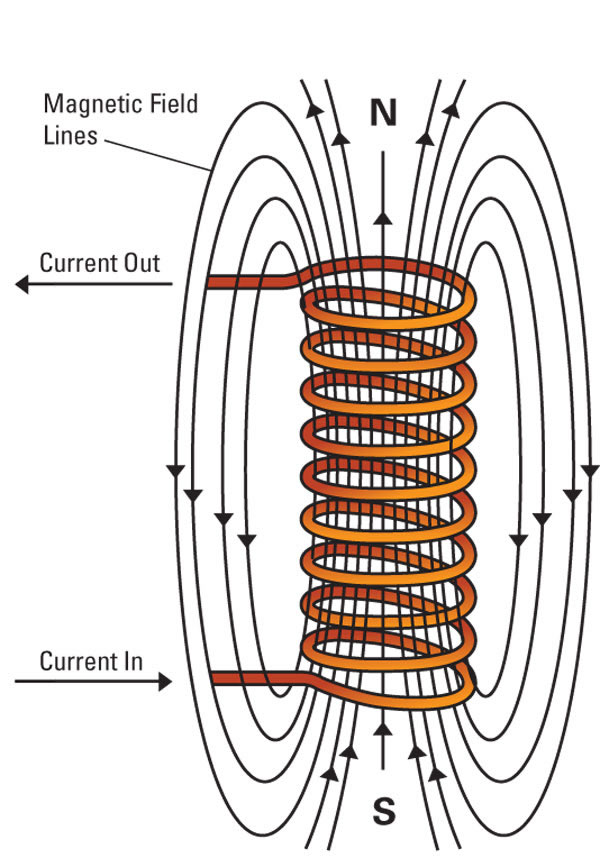
\includegraphics[width=\linewidth]{FigurasMemoria/fig3electromagnet.jpg}
    \caption{Campo magnético en una bobina. www.lanl.gov}
    \label{fig:3} %Para referenciar -> \ref{fig:figNum}
\end{figure}

Como se ha mencionado en la introducción, el funcionamiento de una lanzadera electromagnética se basa en la capacidad de las bobinas de generar un flujo magnético cuando se les aplica una corriente, como se puede ver en la. Esto es debido a la ley de Àmpere, que enuncia lo siguiente:

\begin{quote}
    Según la ley de Ampère, la integral de línea del campo magnético \(\mathbf{B}\) alrededor de un lazo cerrado es igual a \(\mu_0\) multiplicado por la corriente total \(I_{enc}\) que pasa a través de cualquier superficie delimitada por el lazo. Matemáticamente, esto se expresa como:
    \[
    \oint_{\partial S} \mathbf{B} \cdot d\mathbf{l} = \mu_0 I_{enc}
    \]
    donde \(\mu_0\) es la permeabilidad del vacío.
\end{quote}

La manera más básica de representar una lanzadera es un simple circuito con una fuente de alimentación, un interruptor controlado por un circuito electrónico y una bobina, que es la encargada de generar el campo.

\newpage
\section{Desarrollo}
\label{sec:desarrollo}

En esta sección se detallarán los pasos llevados a cabo para la consecución del objetivo principal de este proyecto: el diseño y construcción de una \textit{lanzadera electromagnética}. En los siguientes apartados, se describirán concisamente los procedimientos, herramientas y resultados obtenidos en cada una de estas fases del desarrollo.
\subsection{Desarrollo teórico}
\label{subsec:desarrolloteorico}
En la sección de desarrollo teórico trataré de proporcionar un procedimiento mediante el cual los alumnos que realicen la práctica sean capaces de optimizar la velocidad y fuerza del proyectil a partir de los parámetros eléctricos y geométricos que definen el sistema. Estos parámetros de entrada serán:
\begin{itemize}
    \item \textbf{Parámetros geométricos}:
    \begin{enumerate}[label=\alph*., leftmargin=*, itemindent=1em]
        \item \(r_{cext}\) y \(r_{cint} \): radios exterior e interior de la bobina, respectivamente.
        \item \(l_c\): altura de la bobina.
        \item \(r_{fe}\): radio del vástago.
        \item \(l_{fe}\): longitud del vástago.
        \item \(k_{disp}\): parámetro multiplicador para obtener la sección de dispersión. La dispersión es la parte del flujo que abraza a la bobina y a la barra.
    \end{enumerate}
    \item \textbf{Parámetros eléctricos}:
    \begin{enumerate}[label=\alph*., leftmargin=*, itemindent=1em]
        \item \(N\): número de espiras.
        \item \(I_{cc}\): corriente de alimentación del solenoide.
        \item \(\mu_{fe}\): permeabilidad relativa del vástago ferromagnético.
    \end{enumerate}
\end{itemize}

El objetivo de este desarrollo es crear un programa en MATLAB al que se le proporcionen estos datos, y que calcule automáticamente la fuerza que experimentará el proyectil a través del circuito magnético del sistema. Como se muestra en la figura \ref{fig:electromagnet} el valor de \(B\) varía a lo largo del solenoide, por lo tanto, además de los parámetros constantes dados, será necesario parametrizar también la posición del vástago en cada momento (\(x\) en la figura \ref{fig:esquemaDesTeor}) y calcular la fuerza que experimenta en cada una de esas posiciones. Se muesta a continuación el esquema que nos servirá de guía durante la creación del código, en el que se muestran todas las variables mencionadas anteriormente:

\begin{figure}[H]
    \centering
    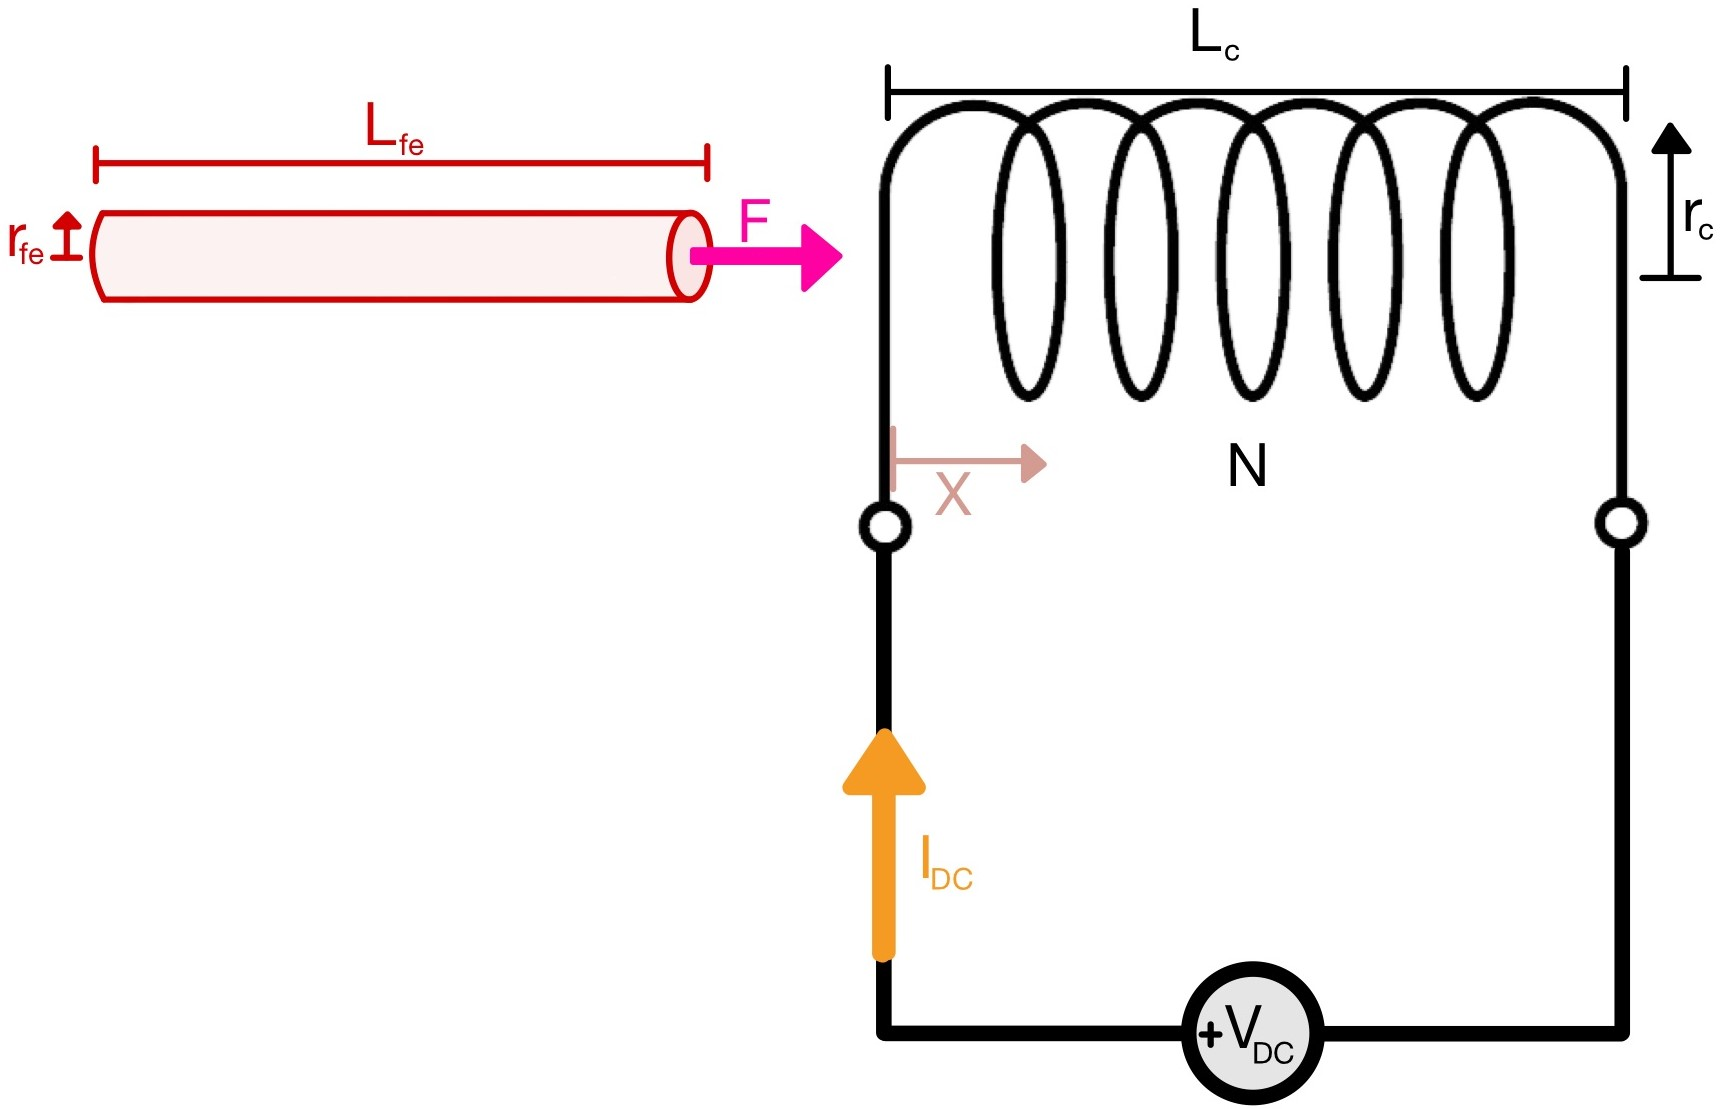
\includegraphics[width=10cm]{FigurasMemoria/esquemaDesTeor.jpg}
    \caption{Esquema geométrico del sistema. Elaboración propia.}
    \label{fig:esquemaDesTeor} %Para referenciar -> \ref{fig:figNum}
\end{figure}

El primer paso será partir de las fórmulas del circuito magnético definidas en el \ref{sec:marcoteorico} marco teórico y para ello la primera tarea es realizar un análisis de las diferentes reluctancias del sistema, con el objetivo de computar así la inducción magnética, la cual nos permitirá obtener la fuerza de atracción que experimenta el vástago, que según Nicolás Jerez \citep{jerez2016resueltos} viene dada por la expresión:

\begin{center}
\[F=\frac{1}{2}\frac{B^2*S}{\mu_0}\]
\end{center}

Teniendo clara la relación entre inducción y fuerza, el siguiente paso es definir claramente las diferentes áreas efectivas de los componentes del sistema para calcular las reluctancias, las cuales son:

\begin{itemize}
    \item \(S_{c}=\pi *r_{cext}^2\): Esta superficie se corresponde con la sección delimitada por el radio exterior de la bobina, y es el área efectiva del flujo encerrado en su interior.
    \item \(S_{fe}=\pi *r_{fe}^2\): Esta superficie se corresponde con la sección delimitada por el radio del vástago.
    \item \(S_{disp}=\pi *r_{disp}~~\forall r_{disp} = k_{disp}r_c\): Esta superficie se corresponde con el área de dispersión de flujo.
\end{itemize}

\begin{figure}[H]
    \centering
    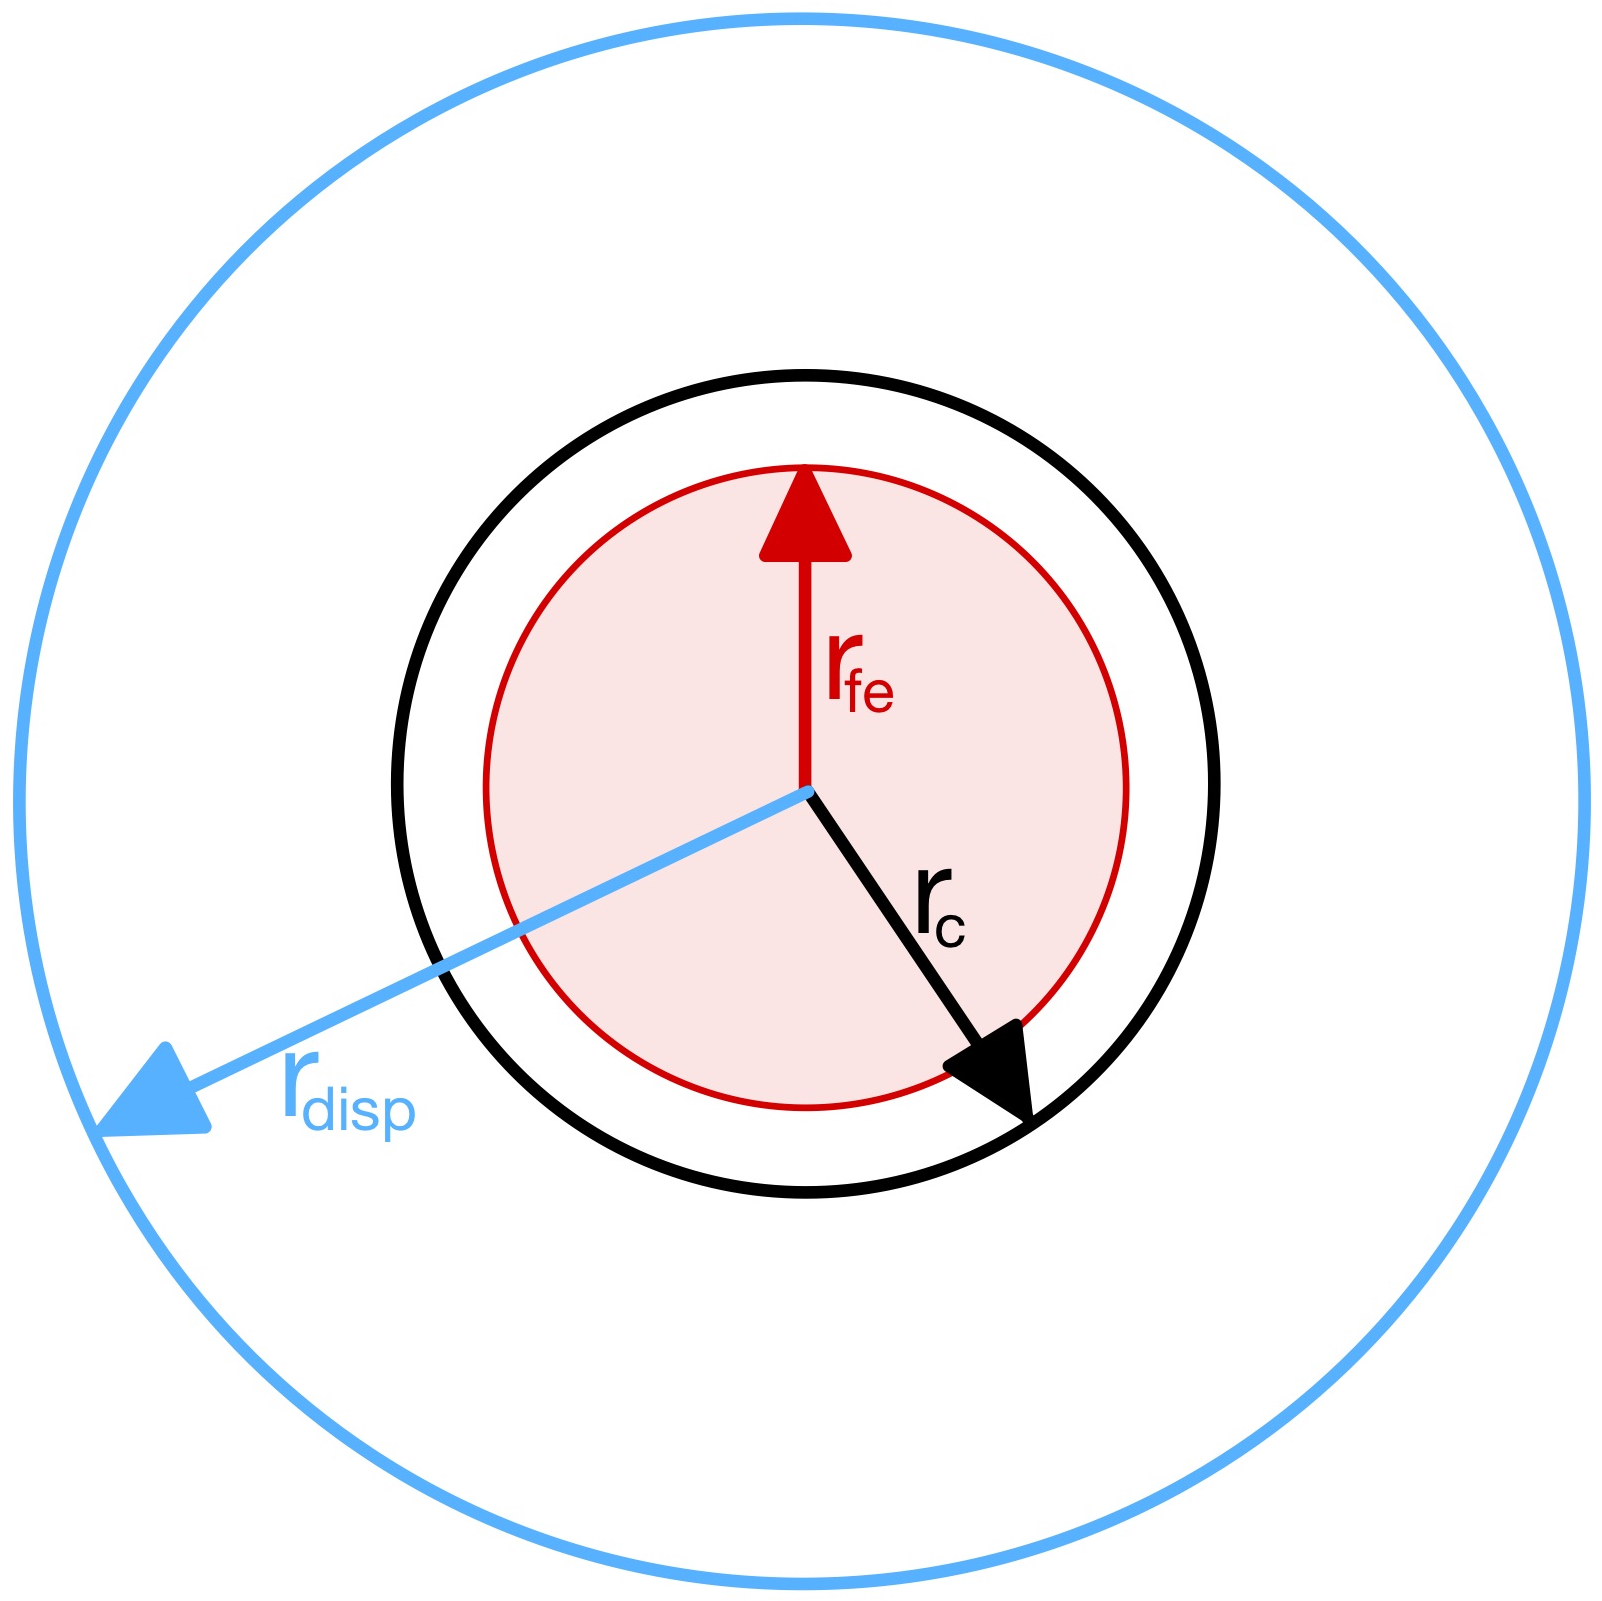
\includegraphics[width=5cm]{FigurasMemoria/areasFlujo.jpg}
    \caption{Secciones del sistema con una vista de planta. Elaboración propia.}
    \label{fig:areasFlujo} %Para referenciar -> \ref{fig:figNum}
\end{figure}

Teniendo en cuenta las fórmulas en la sección del marco teórico (\ref{sec:marcoteorico}) y lo expuesto en la figura \ref{fig:areasFlujo}, podemos concluir que existen cuatro principales reluctancias en el sistema de la figura \ref{fig:esquemaDesTeor}:

\begin{itemize}
    \item \(\mathcal{R}_{disp~c}=\frac{h_c}{\mu_0*S_{disp}}\): Se corresponde a la reluctancia del aire que abraza la bobina. Esta reluctancia es fija ya que las dimensiones del solenoide son constantes.
    \item \(\mathcal{R}_{fe}=\frac{l_{fe}}{\mu_0*\mu_{fe}*S_{fe}}\): Se corresponde a la reluctancia de la barra. Esta reluctancia es fija ya que las dimensiones del vástago son constantes.
    \item \(\mathcal{R}_{\phi}=\frac{(h_c+l_{fe})-x}{\mu_0*S_{disp}}\): Se corresponde a la reluctancia del aire del camino más largo del flujo magnético, y es la que provoca que el campo del electroimán interactúe con el vástago. Es variable ya que la posición del vástago es variable y el camino se reduce con el tiempo.
    \item \(\mathcal{R}_{aire~c}=\frac{h_c-x}{\mu_0*S_c}\): Se corresponde a la reluctancia del aire en el interior de la bobina. Es variable ya que la cantidad de aire disminuye con la posición del vástago.
\end{itemize}

\begin{figure}[H]
    \centering
    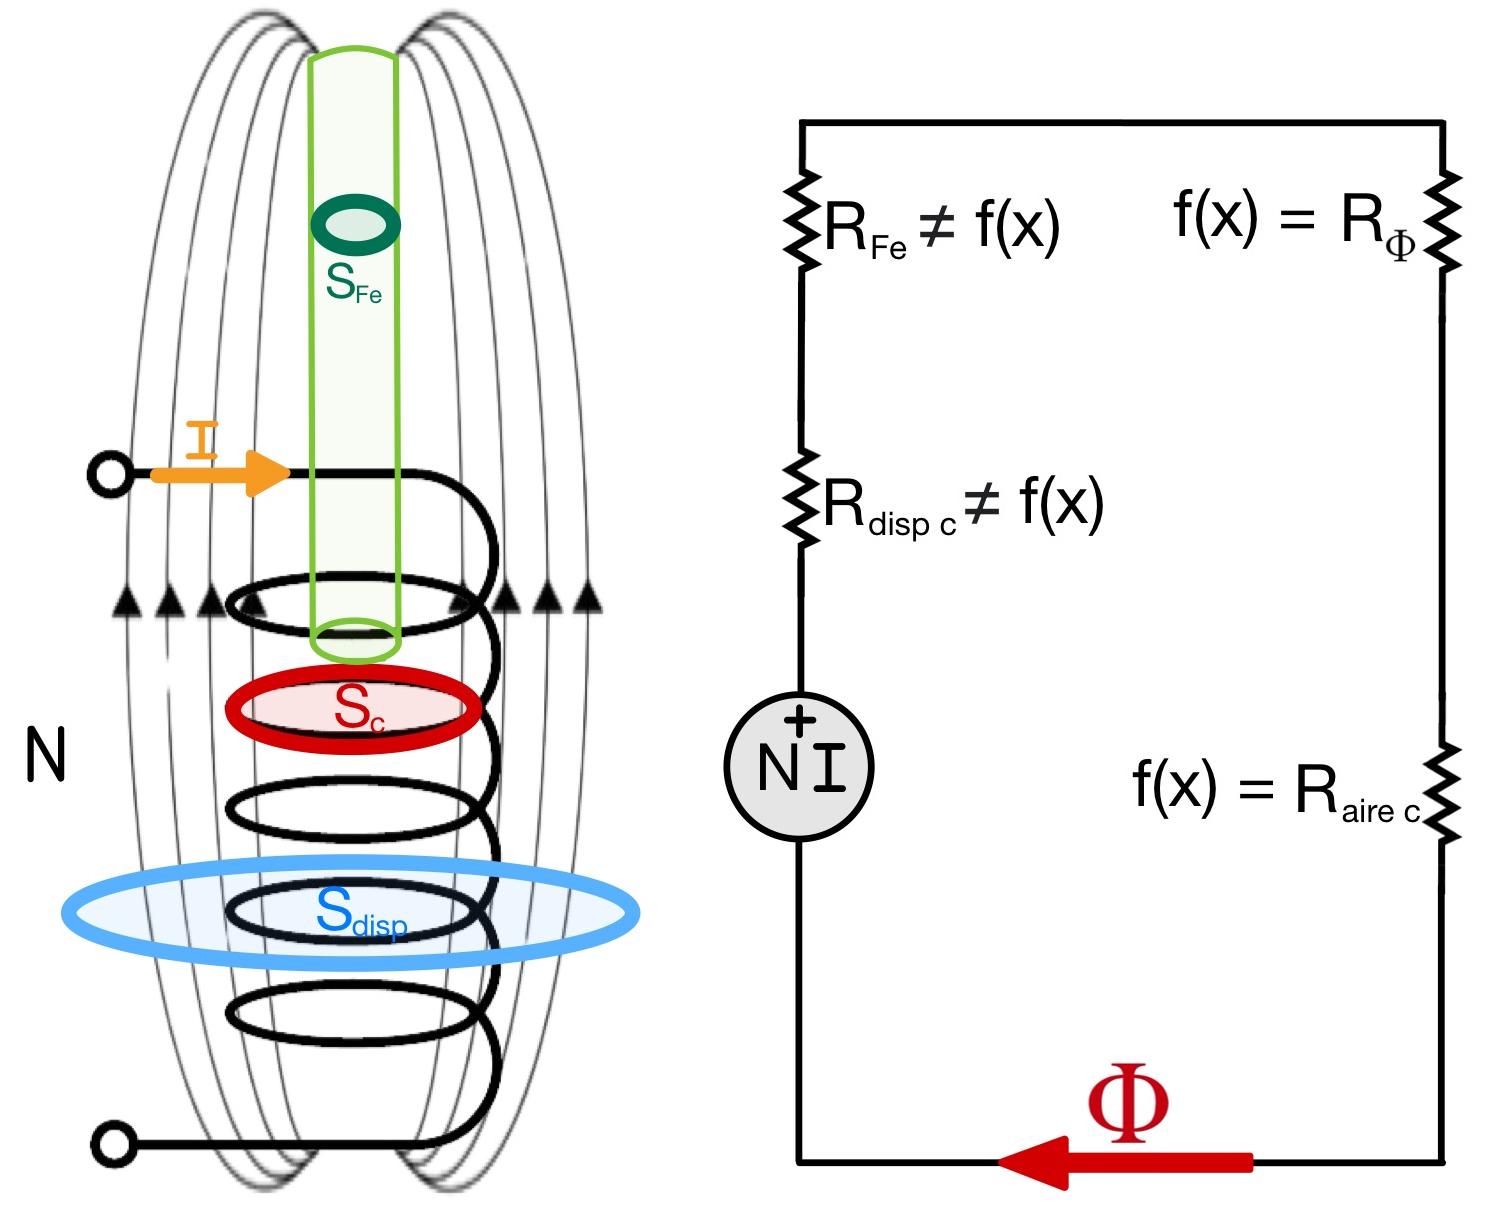
\includegraphics[width=11cm]{FigurasMemoria/circuitoMag.jpg}
    \caption{Circuito magnético del sistema. Elaboración propia.}
    \label{fig:circuitoMag} %Para referenciar -> \ref{fig:figNum}
\end{figure}

\newpage

Con el circuito magnético definido, el siguiente paso es programar las relaciones presentadas en esta sección en MATLAB y graficar los resultados en función de la posición. El programa en MATLAB constará de tres secciones: definición, cálculos y graficación. El código está disonible en el anexo 1 \ref{sec:anexo1}. El producto de este código es una ''calculadora'' que devuelve la evolución de la fuerza con el parámetro \(x\), y queda así:

\begin{figure}[H]
    \centering
    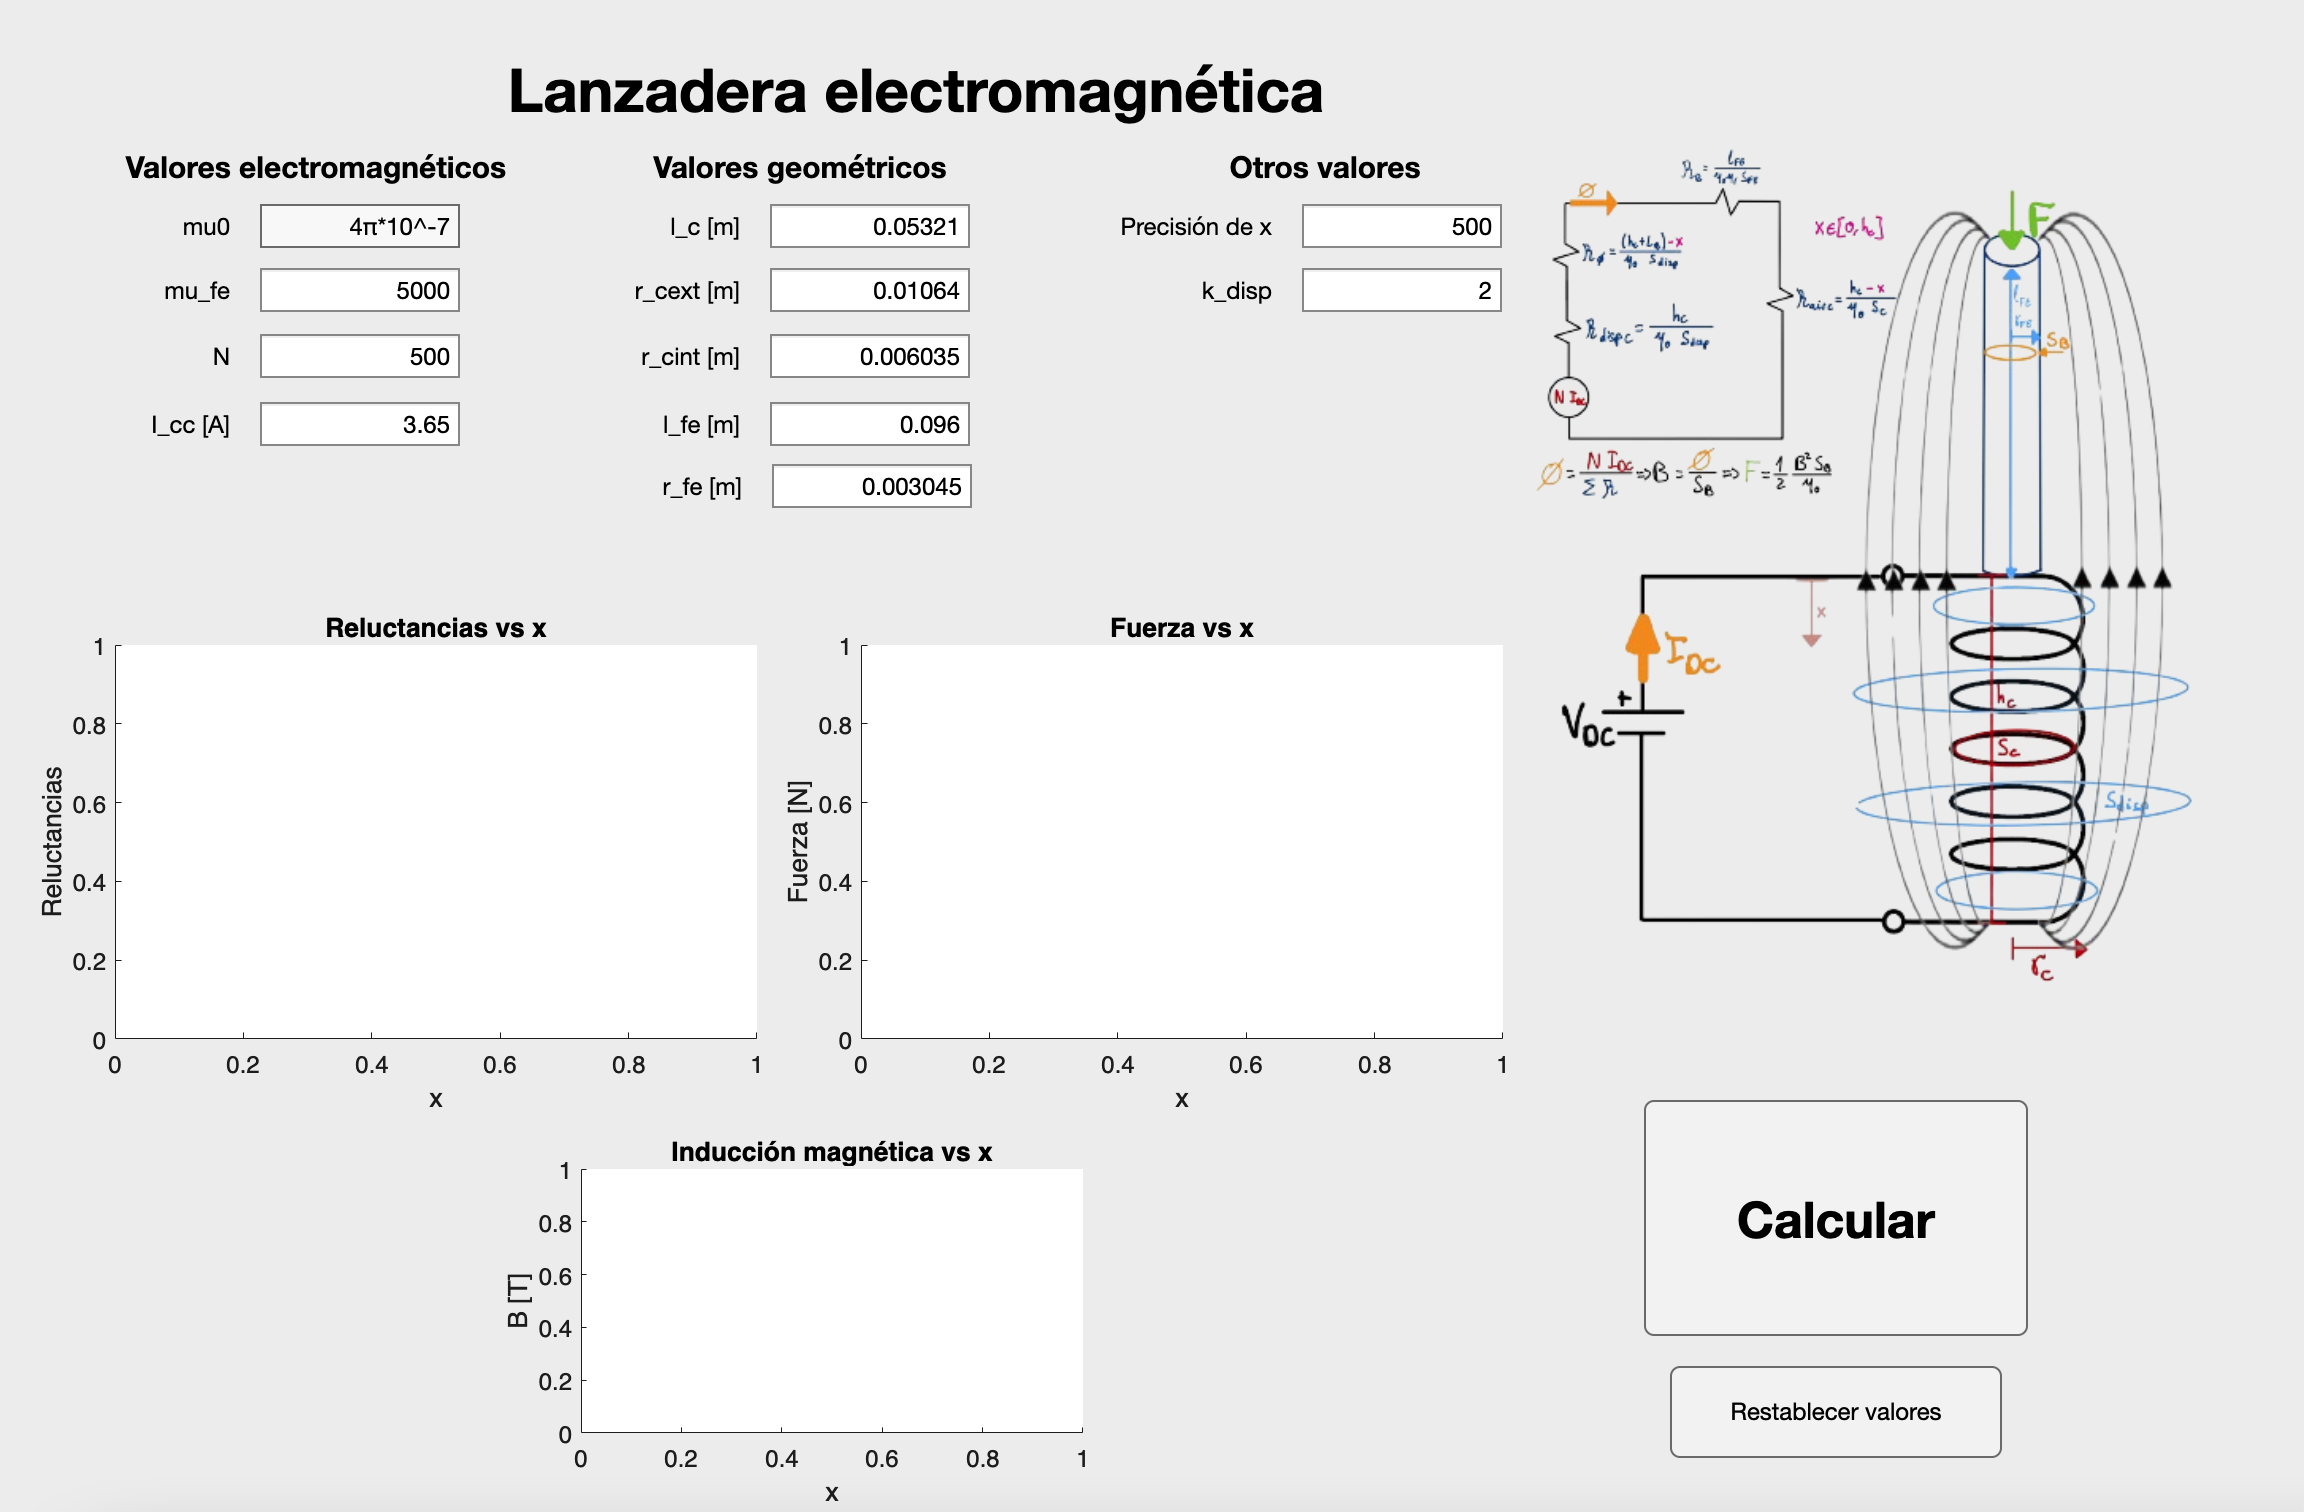
\includegraphics[width=13cm]{FigurasMemoria/calculadora.png}
    \caption{Aplicación de cálculos de MATLAB. Elaboración propia.}
    \label{fig:calculadora} %Para referenciar -> \ref{fig:figNum}
\end{figure}

Los valores escritos en las variables del sistema que se pueden ver en la figura \ref{fig:calculadora} se correponden con la bobina de ejemplo que se ha utilizado para crear el proyecto. Dicha bobina tiene la siguiente geometría:

\[
\begin{array}{c}
    \mu_0 = 4\pi \times 10^{-7}~~~~~~\mu_{fe} = 5000~~~~~~N = 500 \\
    l_{fe} = 0.096m~~~~~~r_{fe} = 0.003045m \\
    h_c = 0.05321m~~~~~~r_{c} = 0.01064m~~~~~~r_{disp} = k_{disp}~r_{c}=2~r_{c}
\end{array}
\]

Con esta configuración, la forma de las gráficas obtenidas es:

\begin{figure}[H]
    \centering
    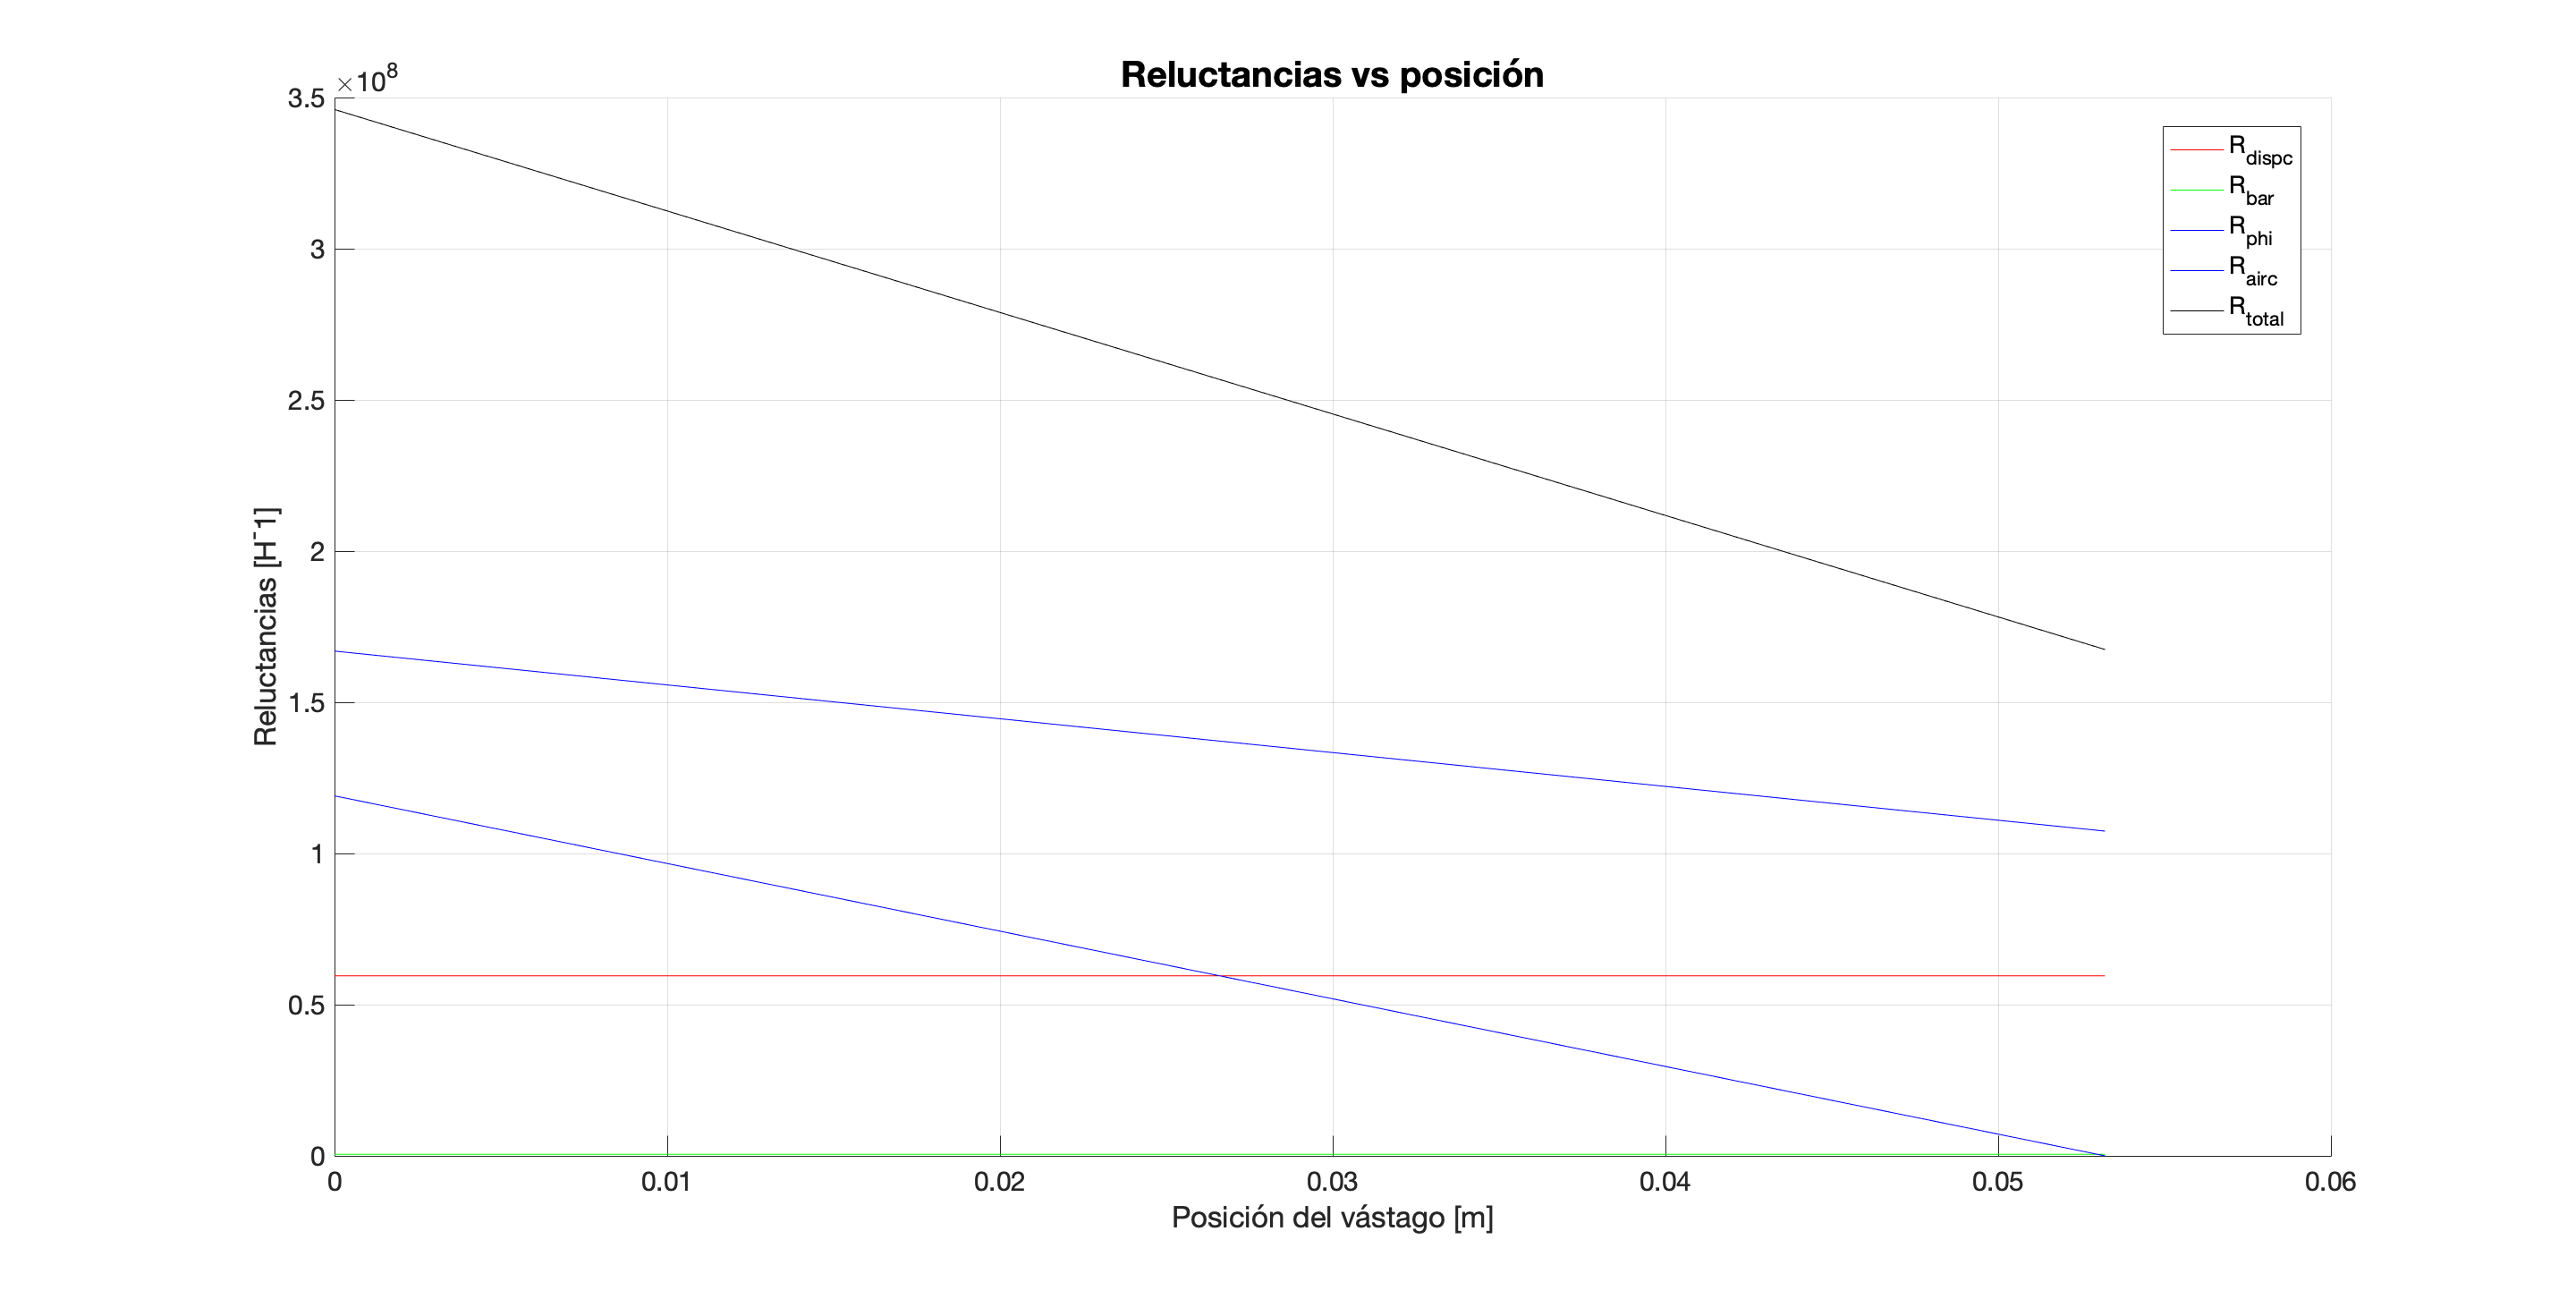
\includegraphics[width=13cm]{FigurasMemoria/calcRsetupBase.png}
    \caption{Reluctancias vs x. Elaboración propia.}
    \label{fig:calcRsetupBase} %Para referenciar -> \ref{fig:figNum}
\end{figure}

\begin{figure}[H]
    \centering
    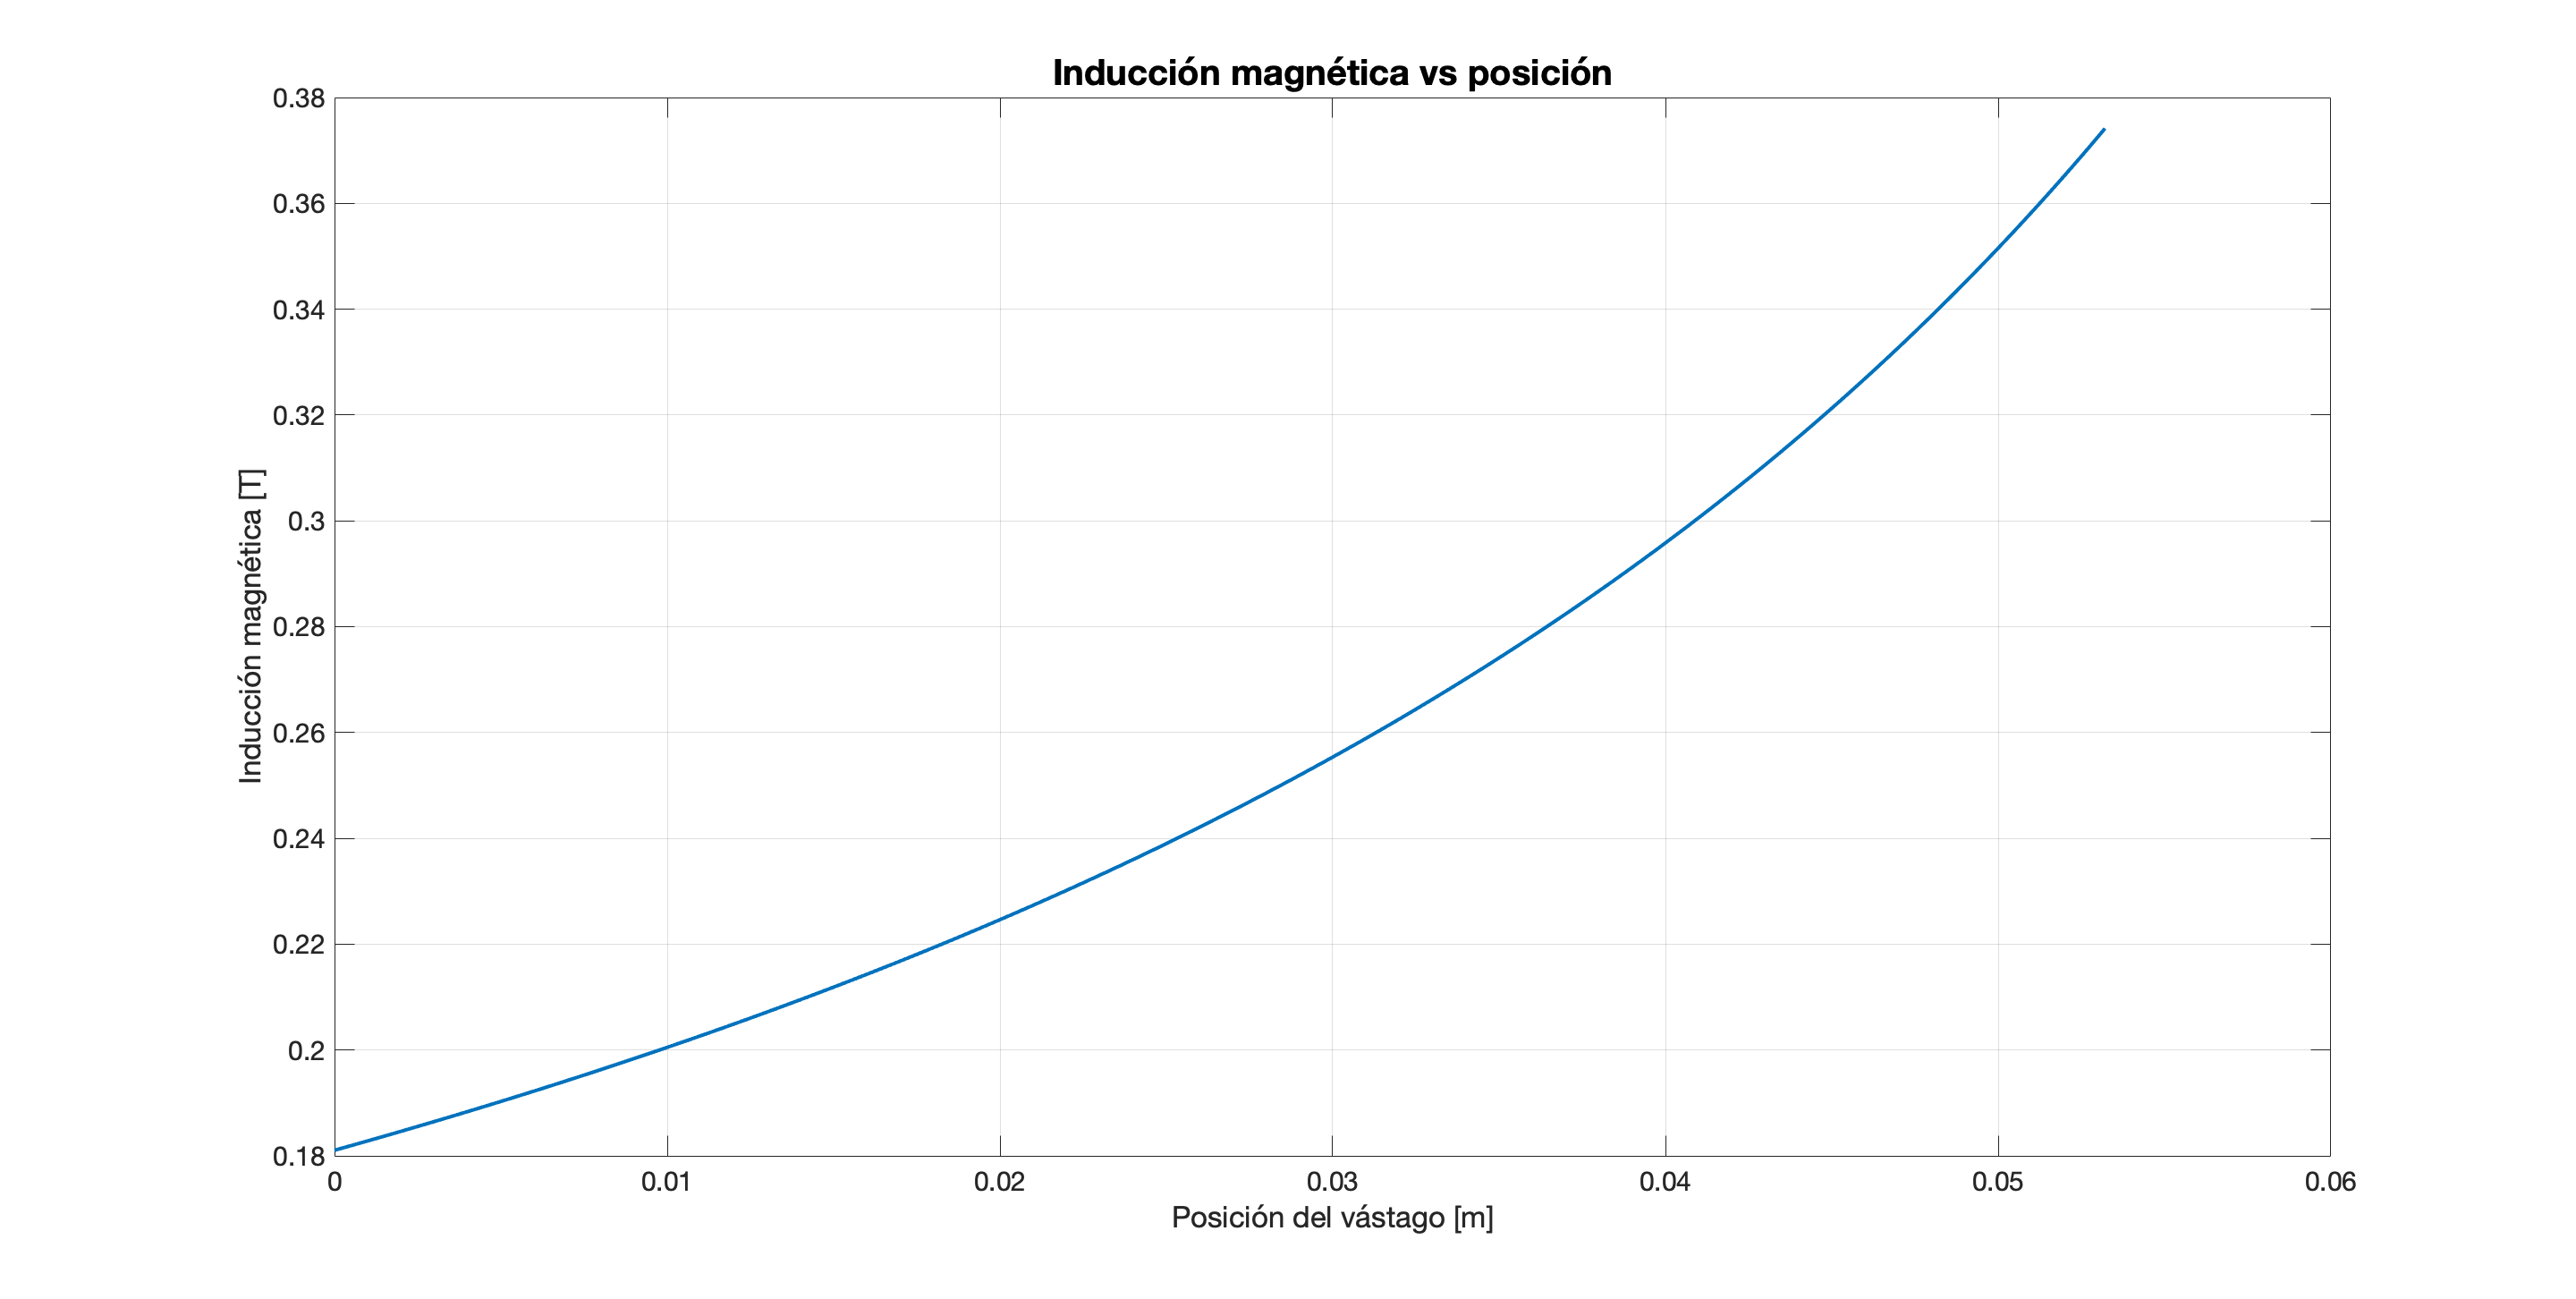
\includegraphics[width=\linewidth]{FigurasMemoria/calcBsetupBase.png}
    \caption{Inducción vs x. Elaboración propia.}
    \label{fig:calcBsetupBase} %Para referenciar -> \ref{fig:figNum}
\end{figure}

\begin{figure}[H]
    \centering
    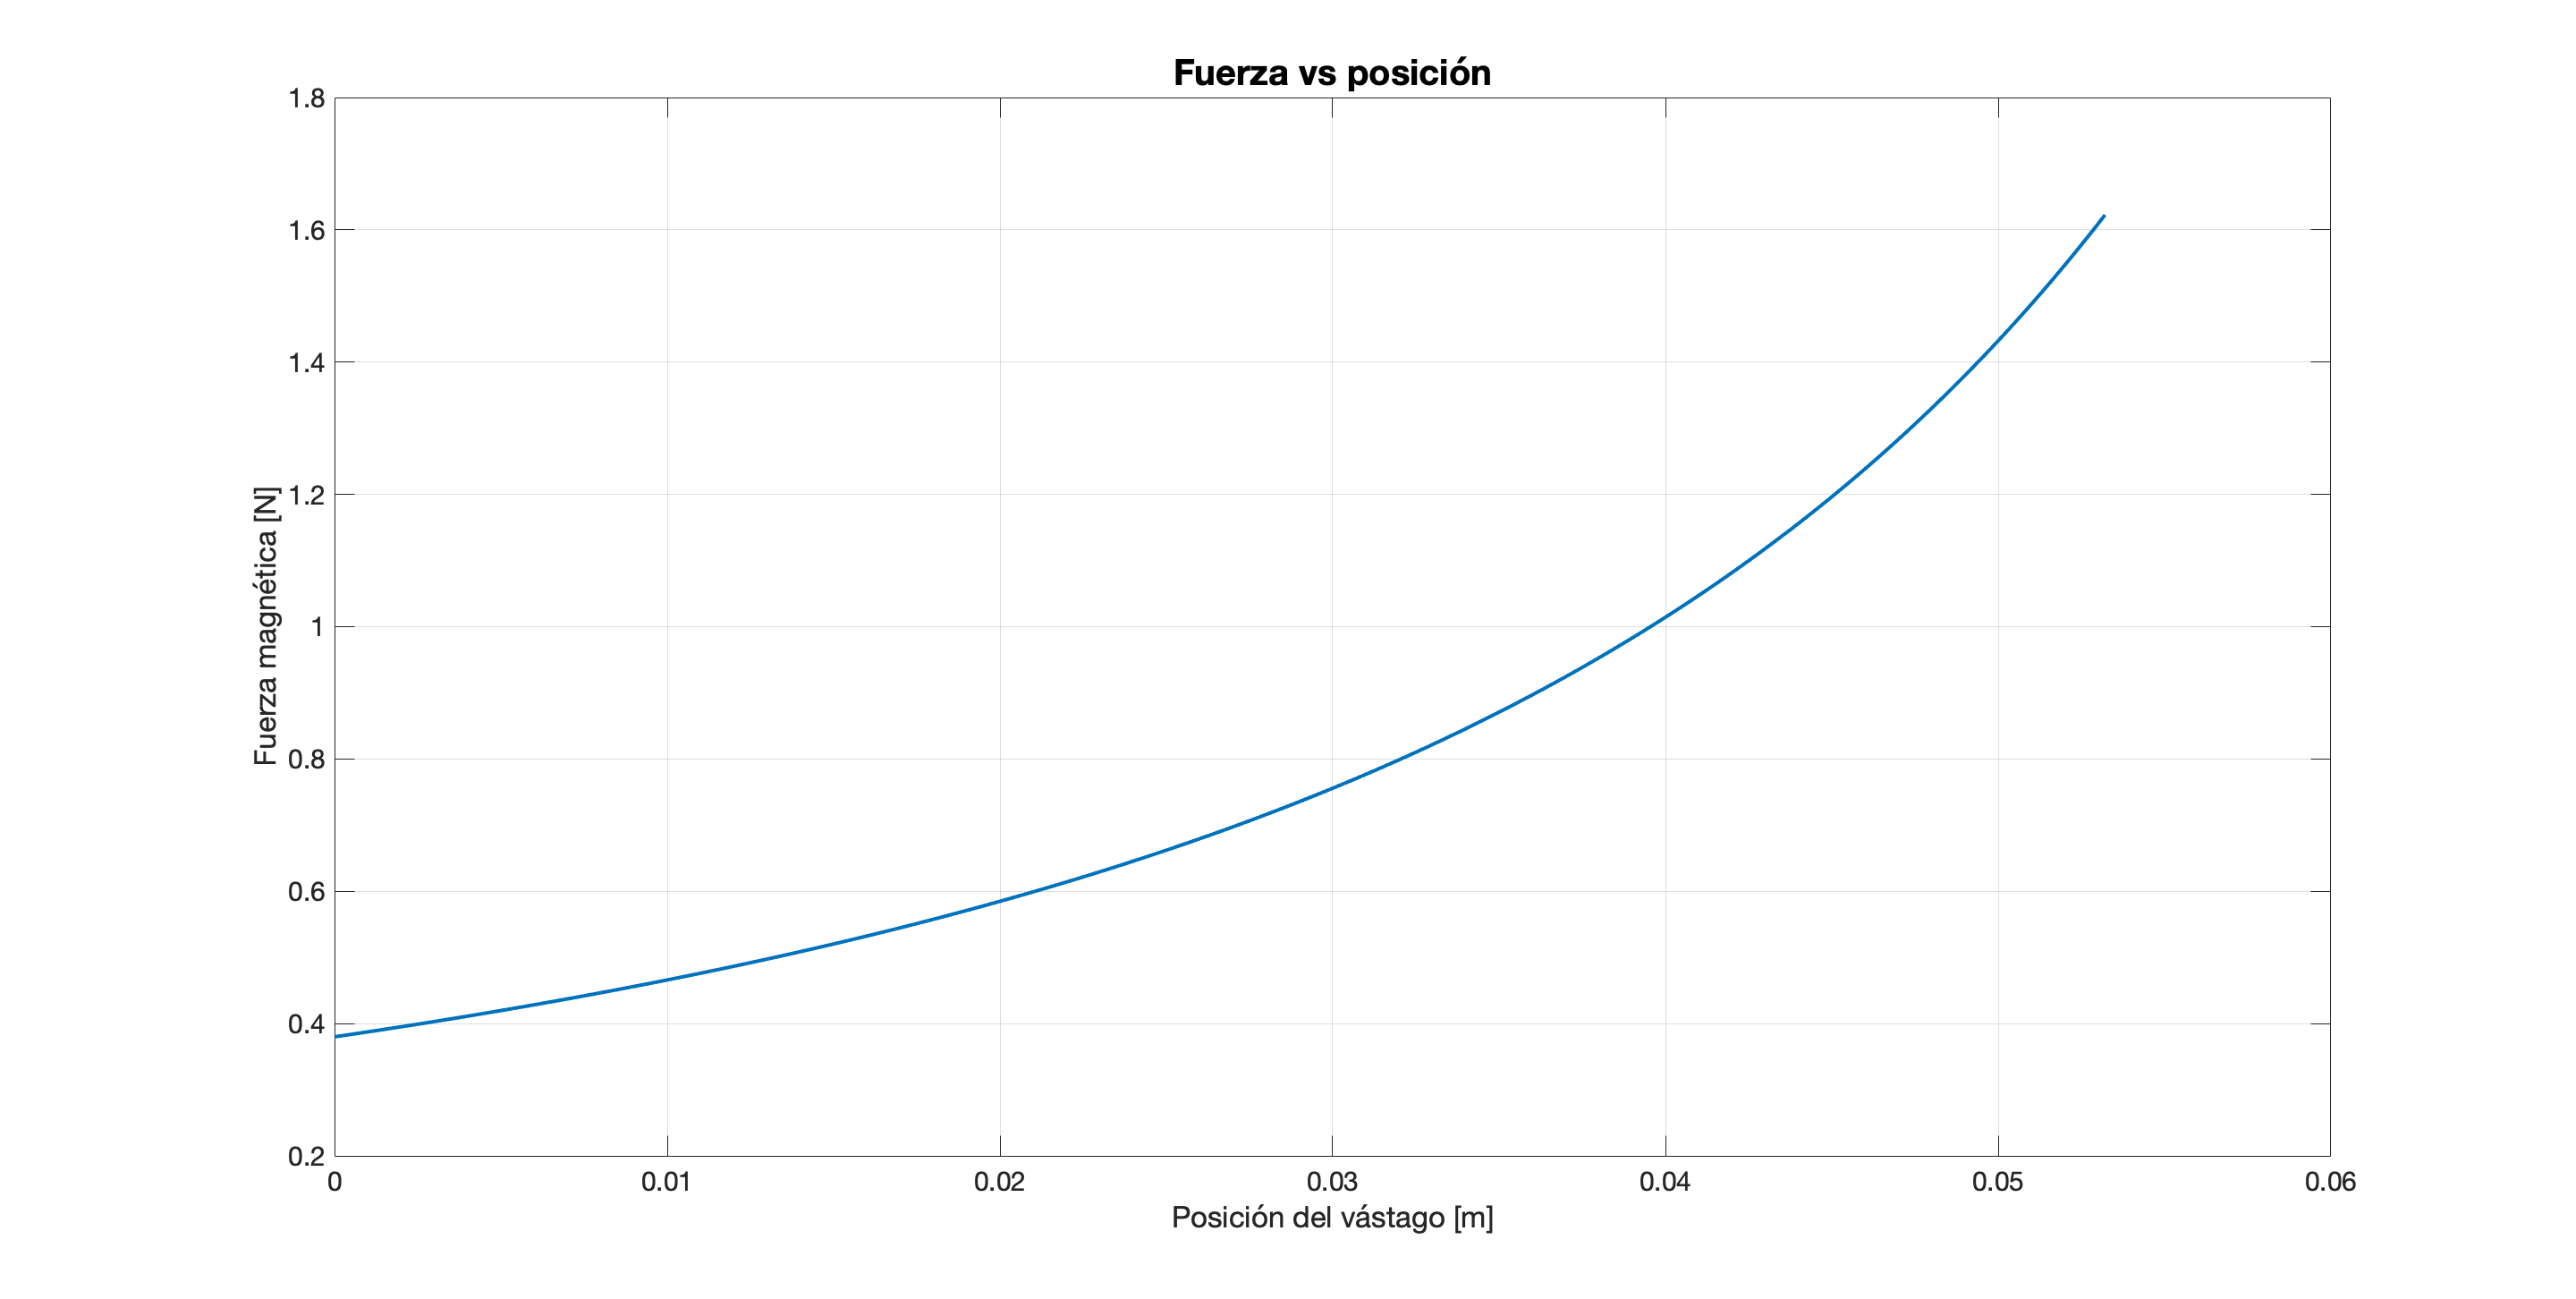
\includegraphics[width=\linewidth]{FigurasMemoria/calcFsetupBase.png}
    \caption{Fuerza vs x. Elaboración propia.}
    \label{fig:calcFsetupBase} %Para referenciar -> \ref{fig:figNum}
\end{figure}

Estas figuras serán discutidas en el apartado de conclusiones %\ref{sec:conclusiones}.

\noindent \textbf{Prueba inicial}
\\~\\
\indent Antes de continuar con el desarrollo, se ha realizado una prueba con un dinamómetro sobre la bobina de prueba especificada anteriormente, para verificar los resultados de la figura \ref{fig:calcFsetupBase} y poder continuar con las simulaciones y prototipo con una referencia. Se ha obtenido el siguiente resultado:

\textbf{HACE FALTA PONER FIGURA CON FOTO DEL DINAMÓMETRO???}

\[F_{vas}=2.4~N~\forall I_{cc}=3.5~A\]

\newpage
\section{Cálculo por Elementos Finitos de la fuerza de atracción}
\label{sec:simulaciones}

En esta sección, se describe el proceso de creación del modelo de la lanzadera electromagnética realizado utilizando ANSYS Maxwell\textsuperscript{\textregistered}. Este software de métodos finitos está especializado en el análisis de sistemas electromagnéticos. El objetivo de estas simulaciones es obtener una comprensión detallada del comportamiento del campo magnético generado por la bobina y su interacción con el proyectil ferromagnético en la lanzadera electromagnética. Se ha dividido el proceso en tres subapartados: creación de la geometría, simulaciones instantáneas y simulaciones transitorias. En la primera, se mostrará el proceso de creación de la geometría paramétrica en 2D y 3D, en la segunda y tercera se explicarán las condiciones de contorno y resultados de las simulaciones instantáneas y transitorias, respectivamente. En el Anexo III se detalla el procedimiento de creación de la geometría y realización de simulaciones.

\subsection{Geometría}
El primer paso para realizar las simulaciones fue la creación de la geometría del sistema en ANSYS Maxwell\textsuperscript{\textregistered}. Para ello, se definieron las dimensiones y características de la bobina y el proyectil de manera paramétrica. Esto quiere decir que las dimensiones de los polígonos que conforman el modelo no son fijas, si no que están asociadas a variables por lo que simular diferentes configuraciones se convierte en algo más sencillo. La geometría fue primeramente diseñada en 3D, pero también se obtuvo la sección central del archivo tridimensional para poder simular en 2D, lo que permite realizar las simulaciones con un menor tiempo de computación. Una vez creada la geometría, se definieron los diferentes materiales y sus propiedades electromagnéticas. El material utilizado para los conductores del solenoide es cobre recocido, PVC para el soporte de la bobina y acero F114 para el vástago. Con esto, se modela la geometría a continuación mostrada:

\begin{itemize}
    \item \textbf{Geometría en 3D}:
    \begin{figure}[H]
        \centering
        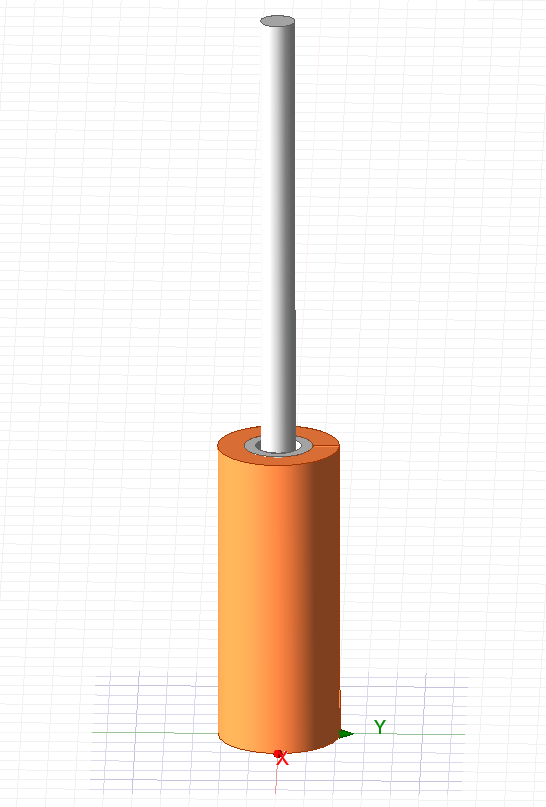
\includegraphics[width=7cm]{FigurasMemoria/geom3d.png}
        \caption{Geometría de la barra y bobina en 3D.}
        \label{fig:geom3d} %Para referenciar -> \ref{fig:figNum}
    \end{figure}
    \item \textbf{Mallado en 3D}:
    \begin{figure}[H]
        \centering
        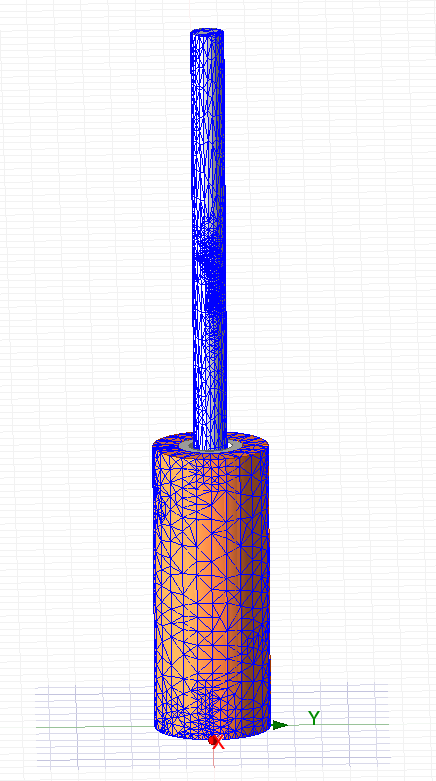
\includegraphics[width=7cm]{FigurasMemoria/mesh3d.png}
        \caption{Mallado de la barra y bobina en 3D.}
        \label{fig:mesh3d} %Para referenciar -> \ref{fig:figNum}
    \end{figure}
    \begin{figure}[H]
        \centering
        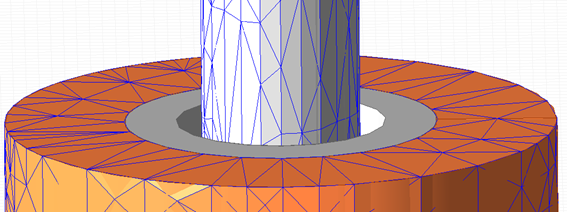
\includegraphics[width=9cm]{FigurasMemoria/meshDetail3d.png}
        \caption{Detalle del mallado de la barra y bobina en 3D.}
        \label{fig:meshDetail3d} %Para referenciar -> \ref{fig:figNum}
    \end{figure}

    \vspace{5cm}
    
    \item \textbf{Geometría en 2D}:
    \begin{figure}[H]
        \centering
        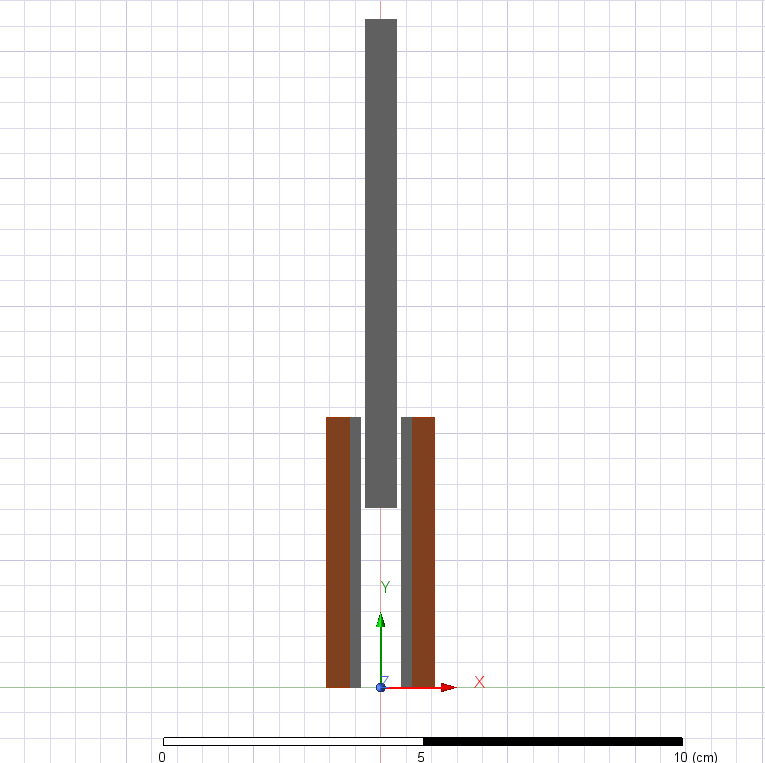
\includegraphics[width=9cm]{FigurasMemoria/BarGeom.png}
        \caption{Geometría de la barra y bobina en 2D.}
        \label{fig:BarGeom} %Para referenciar -> \ref{fig:figNum}
    \end{figure}
    \item \textbf{Mallado en 2D}
    \begin{figure}[H]
        \centering
        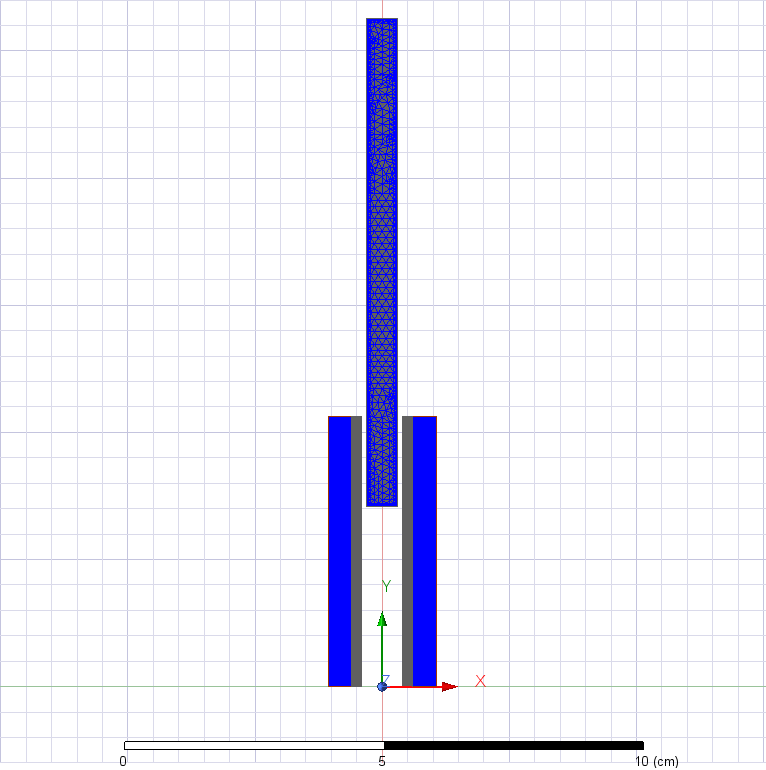
\includegraphics[width=9cm]{FigurasMemoria/BarGeomMesh.png}
        \caption{Mallado de la barra y bobina en 2D.}
        \label{fig:BarGeomMesh} %Para referenciar -> \ref{fig:figNum}
    \end{figure}
    \begin{figure}[H]
        \centering
        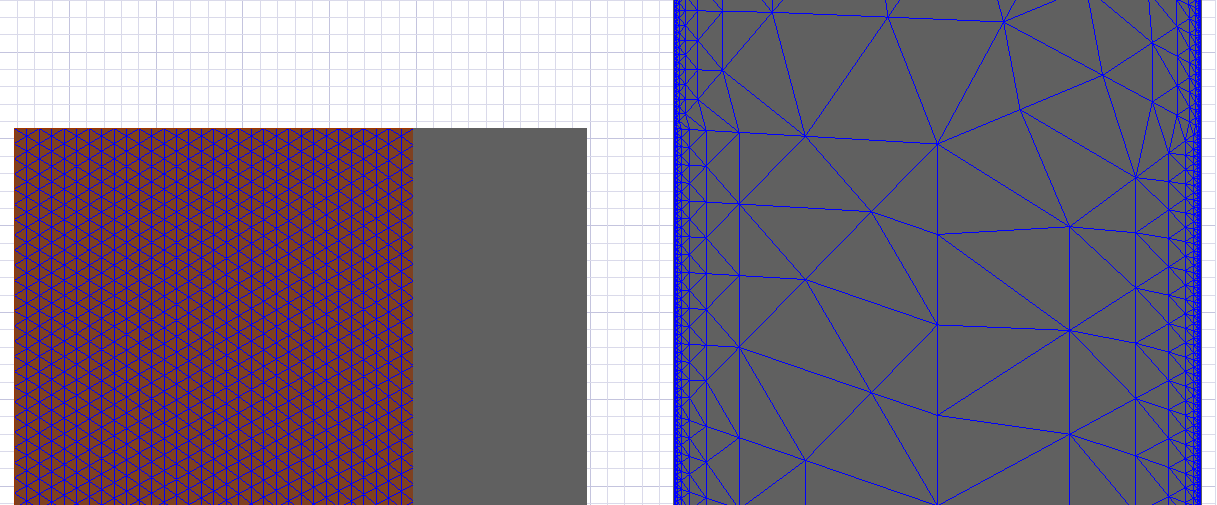
\includegraphics[width=9cm]{FigurasMemoria/BarMeshDetail.png}
        \caption{Detalle del mallado de la barra y bobina en 2D.}
        \label{fig:GeomMeshDetail} %Para referenciar -> \ref{fig:figNum}
    \end{figure}
\end{itemize}

La bobina (cilindro ocre), se ha generado de la manera mostrada y no con un polígono helicoidal debido a que el orden de magnitud de espiras (\(10^2\)) y el orden de magnitud de las medidas (\(10^{-3}\)) convierte esto en una muy compleja tarea, ya que ANSYS Maxwell\textsuperscript{\textregistered} no es un entorno de diseño en 3D. Al crear un cilindro con dimensiones apropiadas, se puede indicar al software que lo trate como un solenoide, asignándole un número de espiras y una corriente de excitación. El programa distribuye uniformemente el campo generado por la corriente en todo el volumen, lo que resulta en una aproximación muy válida de un solenoide, sin necesidad de crear una geometría extremadamente compleja \citep[p. 13]{ansoft2012maxwell}.

\subsection{Simulaciones instantáneas}
ANSYS Maxwell\textsuperscript{\textregistered} permite realizar simulaciones de diferentes tipos, de las cuales tienen interés para este proyecto las magnetoestáticas y las transitorias. Como primera prueba para el modelo de la figura \ref{fig:geom3d}, se realizó una simulación electroestática con una \(I_{cc}=3.65~A\) para poder observar los campos magnéticos del sistema, resultando en la siguiente figura:

\begin{figure}[H]
    \centering
    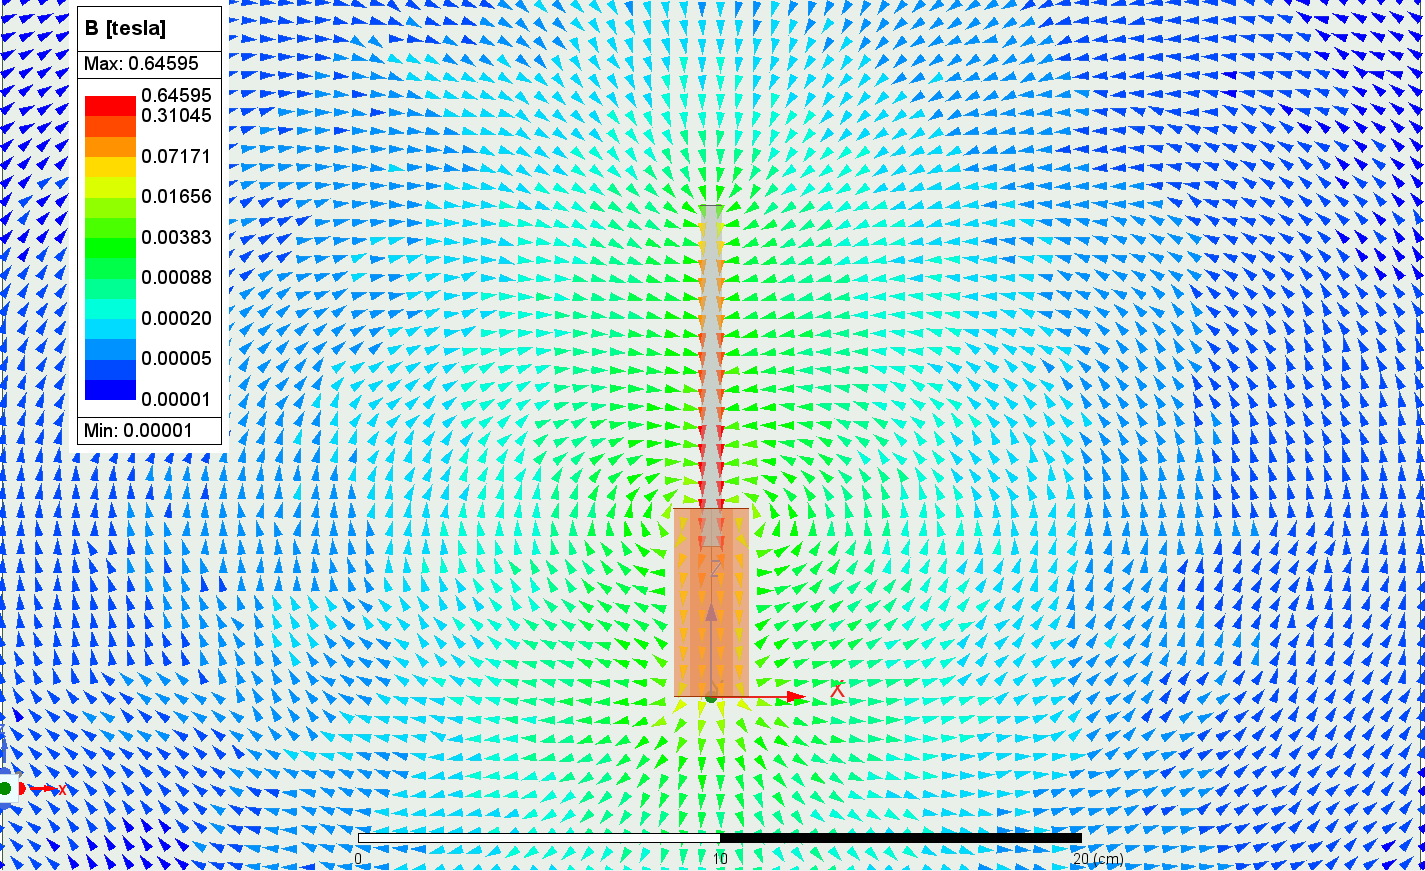
\includegraphics[width=14cm]{FigurasMemoria/fields8.PNG}
    \caption{Visualización de los campos magnéticos con la bobina energizada con \(I_{cc}=3.5~\text{A}\) y \(x=8/10 * h_c\).}
    \label{fig:fields8} %Para referenciar -> \ref{fig:figNum}
\end{figure}

Vemos que se puede apreciar perfectamente la forma descrita en las figuras \ref{fig:integralampere} y \ref{fig:electromagnet}, curvándose en los extremos del sistema pero permaneciendo bastante uniforme a lo largo de \(h_c\). Se muestra a continuación un detalle de los campos únicamente dentro de la bobina con la barra en la posición de la figura \ref{fig:fields8}:

\begin{figure}[H]
    \centering
    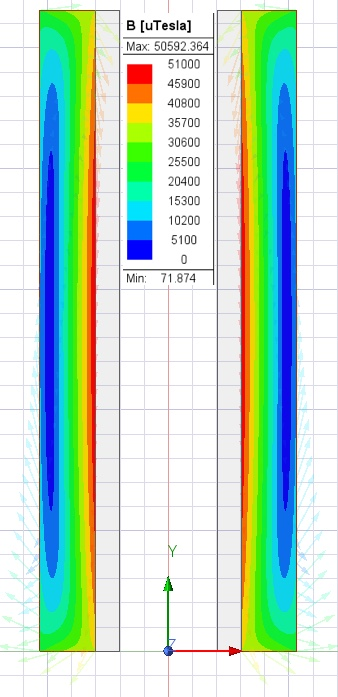
\includegraphics[width=3cm]{FigurasMemoria/fieldsDetail.jpg}
    \caption{Visualización de los campos magnéticos dentro del solenoide.}
    \label{fig:fieldsDetail} %Para referenciar -> \ref{fig:figNum}
\end{figure}

Además de visualizar los campos, ANSYS Maxwell\textsuperscript{\textregistered} permite añadir distintas medidas a la simulación, entre las que se encuentra la fuerza de atracción magnética. Realizando la simulación de nuevo para la configuración en 3D, se obtiene que la fuerza es igual a:

\begin{table}[h]
    \centering
    \begin{tabular}{|c|c|c|c|c|}
        \hline
        & \(F_x\) & \(F_y\) & \(F_z\) & \(F_{tot}\) \\
        \hline
        \(F_{ANSYS}\) & Data 2 & Data 3 & Data 4 & Data 5 \\
        \hline
    \end{tabular}
    \caption{Fuerzas de atracción magnética en los diferentes ejes del espacio.}
    \label{tab:fuerzas}
\end{table}

\subsection{Simulaciones transitorias}
Una vez observados los campos de manera estacionaria, el siguiente paso es conseguir la variación de los valores de fuerza con la posición del vástago, además sin forzar este movimiento. Es decir, especificar la región de movimiento y los valores de alimentación de la bobina y dejar que ANSYS Maxwell\textsuperscript{\textregistered} genere el movimiento y nos de información acerca de la fuerza y velocidad experimentadas por el vástago. Al realizar esto con el modelo 3D, ANSYS Maxwell\textsuperscript{\textregistered} devolvía un error fatal probablemente debido a que los ordenadores en los que se estaba realiando la simulación no eran lo suficientemente potentes. Se recurrió entonces a la utilización exclusiva de la geometría en 2D, la que dio resultados tanto de movimiento como fuerza. Para llegar a los últimos resultados, se realizaron varias simulaciones con varias configuraciones temporales diferentes, las cuales se muestran a continuación:
\subsection*{Configuración 1}
La primera configuración transitoria utilizada es:
\[
T_{sim}=150~ms \quad T_{step}=5~ms \to 30~steps
\]
\[
I(t=0)=3.5~A \quad I(t\geq 50~ms)=0~A
\]
\[
V_{coil}=13.1~V \quad R_{coil}=3.65~\Omega
\]
\[
m_{bar}=0.019~kg \quad v_{bar~ini}=0~ms^{-1}
\]
Las gráficas resultantes de fuerza-corriente y velocidad-posición son:
\begin{figure}[H]
    \centering
    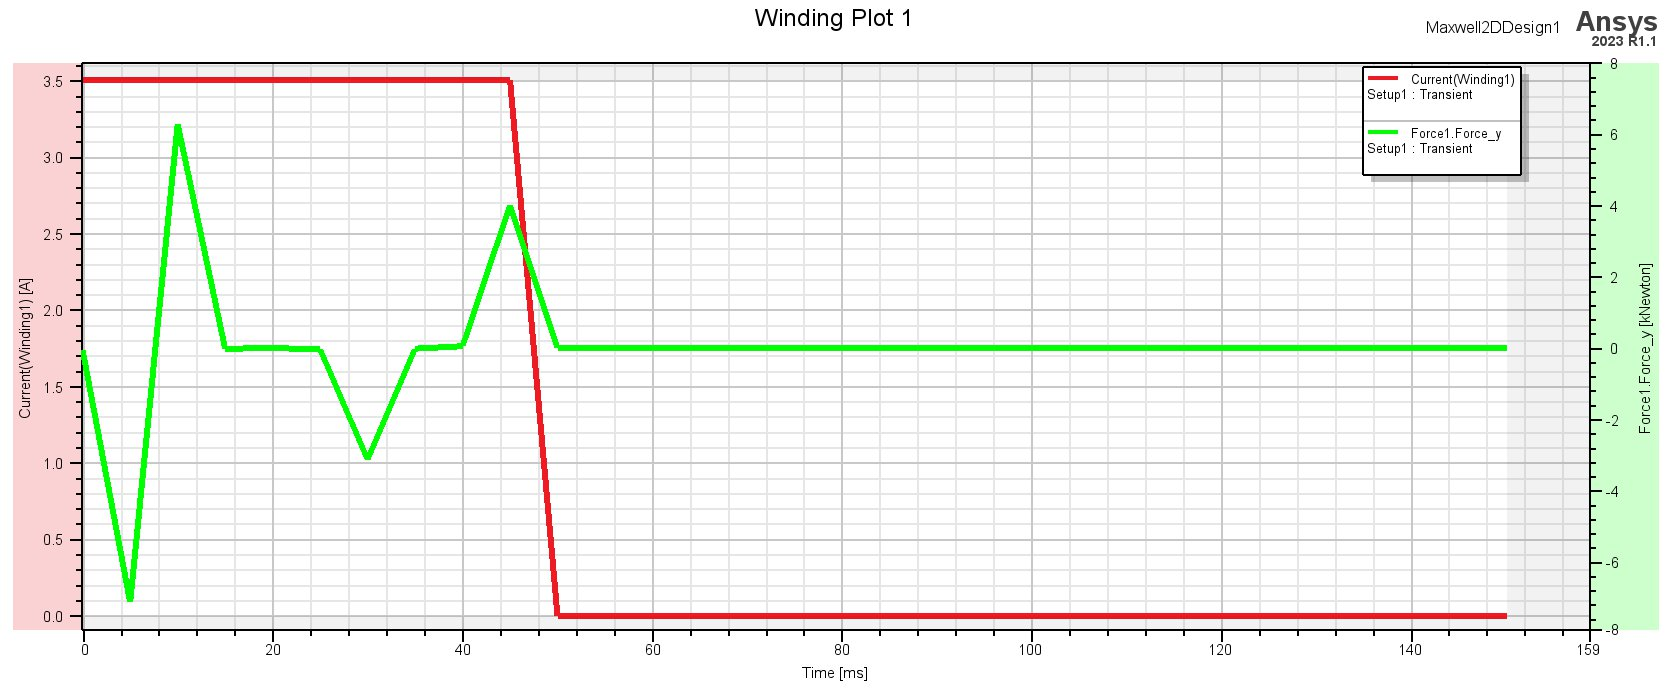
\includegraphics[width=13cm]{FigurasMemoria/S1CurrentForce.jpg}
    \caption{Fuerza (verde) y corriente (rojo) en función del tiempo de la configuración 1.}
    \label{fig:S1CurrentForce} %Para referenciar -> \ref{fig:figNum}
\end{figure}
\begin{figure}[H]
    \centering
    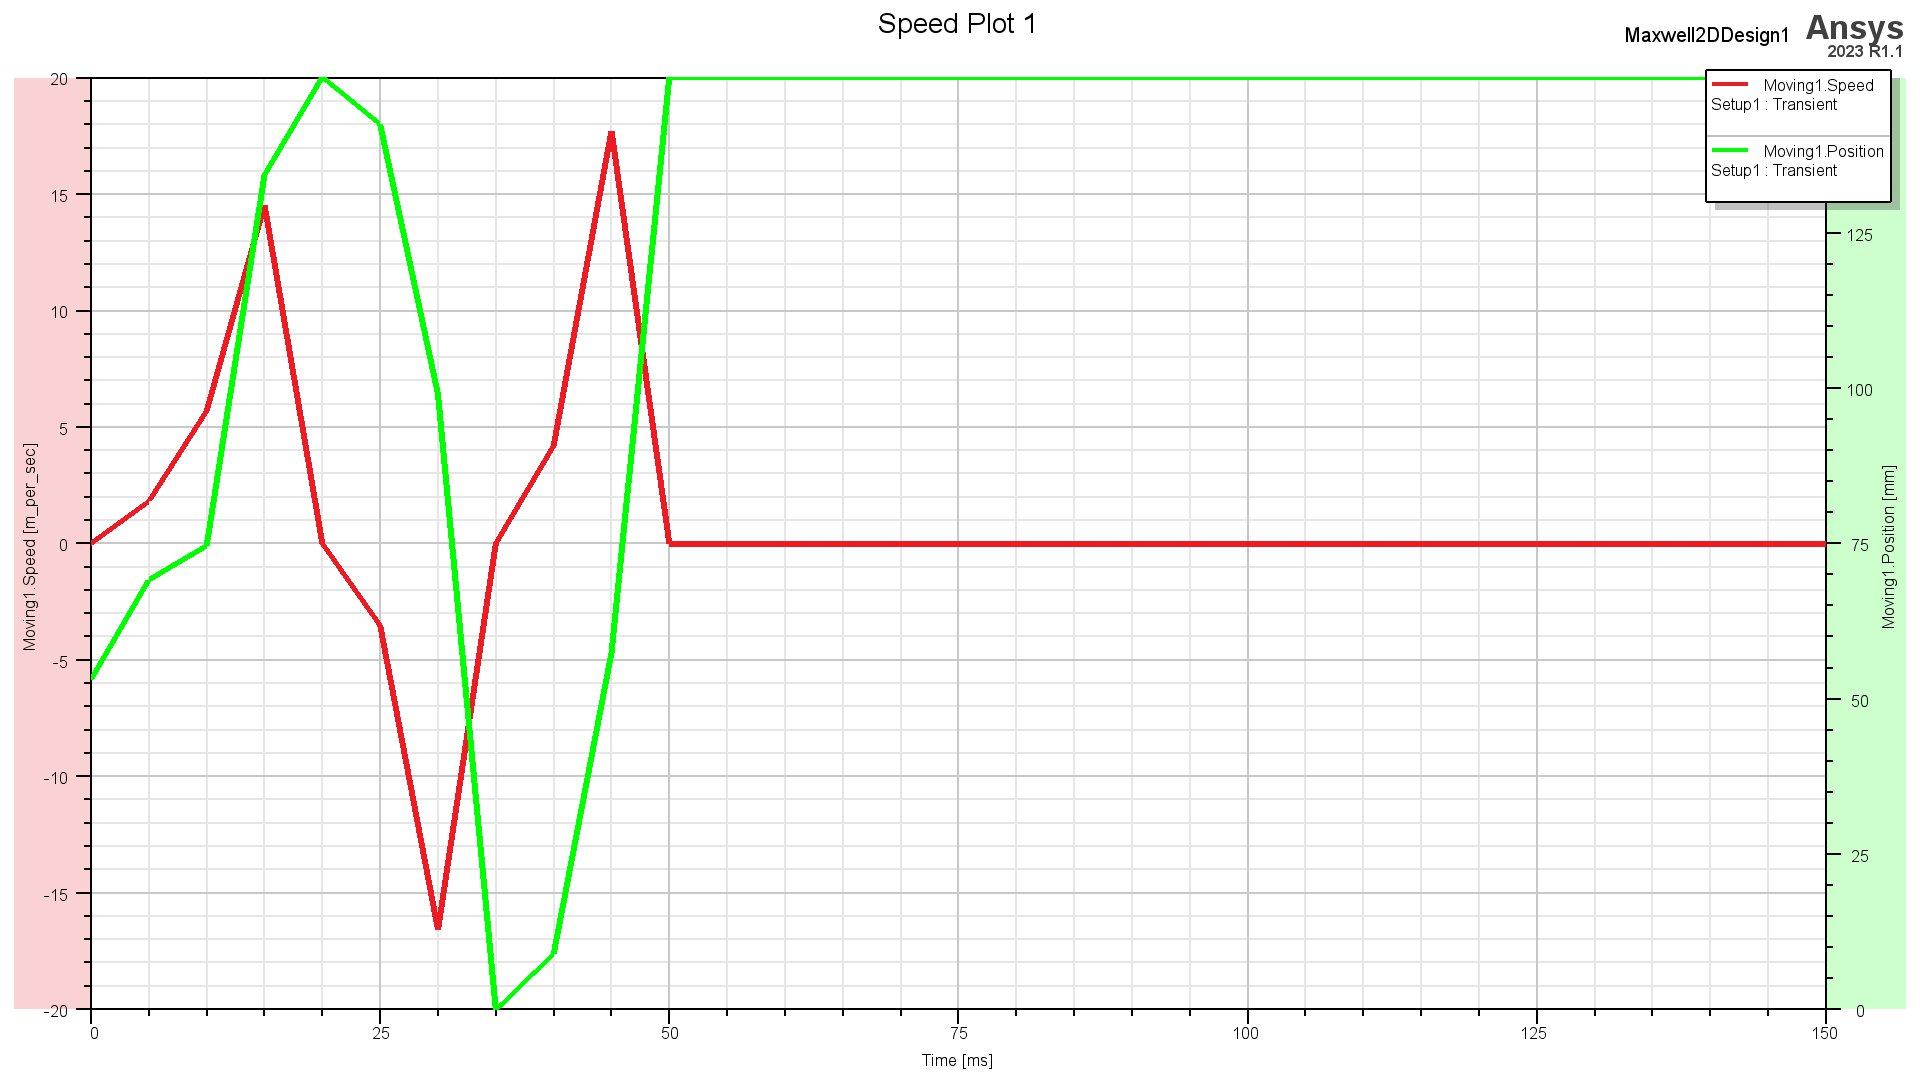
\includegraphics[width=10cm]{FigurasMemoria/S1SpeedPosition.jpg}
    \caption{Posición (verde) y velocidad (rojo) en función del tiempo de en la configuración 1.}
    \label{fig:S1SpeedPosition} %Para referenciar -> \ref{fig:figNum}
\end{figure}
Como se puede observar en las figuras \ref{fig:S1CurrentForce} y \ref{fig:S1SpeedPosition}, \(T_{sim}\) es muy largo ya que la mayor parte del tiempo no ocurre nada. También es destacable que existen oscilaciones, lo que indica que la bobina está siendo alimentada durante demasiado tiempo y está siendo retenida en el centro.


\subsection*{Configuración 2}
La segunda configuración transitoria utilizada es:
\[
T_{sim}=75~ms \quad T_{step}=0.6~ms \to 125~steps
\]
\[
I(t=0)=3.5~A \quad I(t\geq 30~ms)=0~A
\]
\[
V_{coil}=13.1~V \quad R_{coil}=3.65~\Omega
\]
\[
m_{bar}=0.019~kg \quad v_{bar~ini}=0~ms^{-1}
\]
Las gráficas resultantes de fuerza-corriente y velocidad-posición son:
\begin{figure}[H]
    \centering
    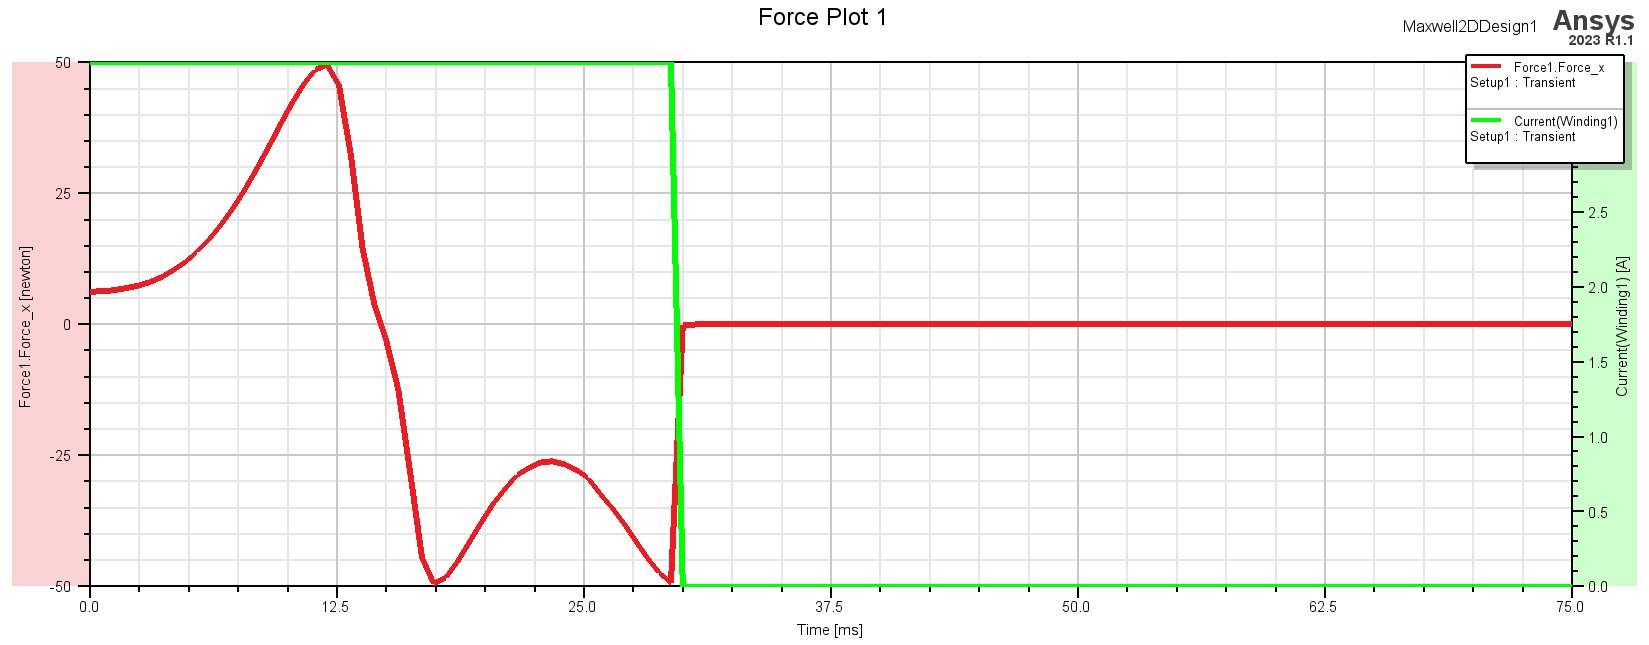
\includegraphics[width=13cm]{FigurasMemoria/S2ForceCurrent.jpg}
    \caption{Fuerza (rojo) y corriente (verde) en función del tiempo de la configuración 2.}
    \label{fig:S2ForceCurrent} %Para referenciar -> \ref{fig:figNum}
\end{figure}
\begin{figure}[H]
    \centering
    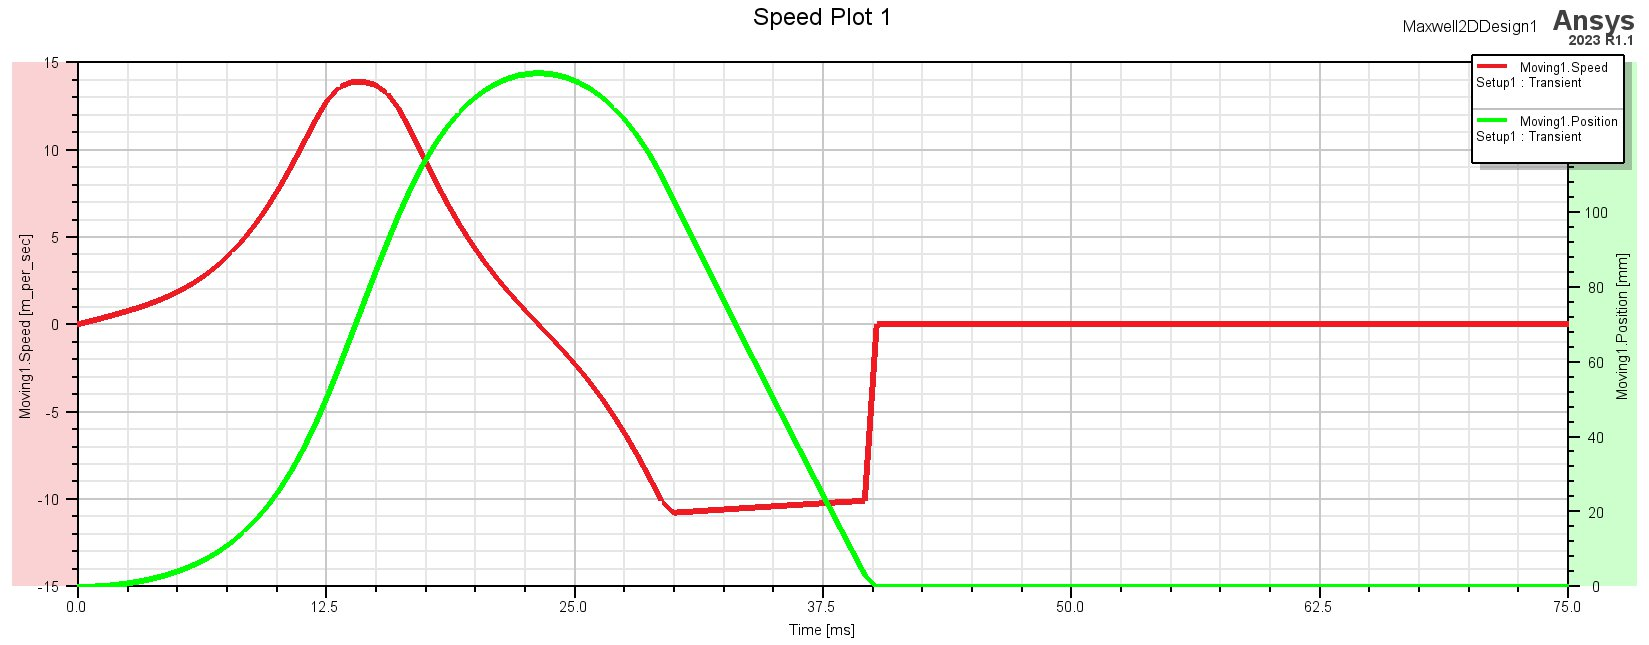
\includegraphics[width=13cm]{FigurasMemoria/S2SpeedPosition.jpg}
    \caption{Posición (verde) y velocidad (rojo) en función del tiempo de la configuración 2.}
    \label{fig:S2SpeedPosition} %Para referenciar -> \ref{fig:figNum}
\end{figure}
En la segunda configuración, se utilizó un timestep muy pequeño para poder observar con precisión el movimiento del vástago. Se observa más ajustado el tiempo de simulación, aunque el tiempo de alimentación de la bobina sigue siendo muy elevado ya que el vástago sigue oscilando, aunque ya solo lo hace una vez. 

\subsection*{Configuración 3}
La tercera configuración transitoria utilizada es:
\[
T_{sim}=25~ms \quad T_{step}=1~ms \to 25~steps
\]
\[
I(t=0)=3.5~A \quad I(t\geq 15~ms)=0~A
\]
\[
V_{coil}=13.1~V \quad R_{coil}=3.65~\Omega
\]
\[
m_{bar}=0.019~kg \quad v_{bar~ini}=0~ms^{-1}
\]
Las gráficas resultantes de fuerza-corriente y velocidad-posición son:
\begin{figure}[H]
    \centering
    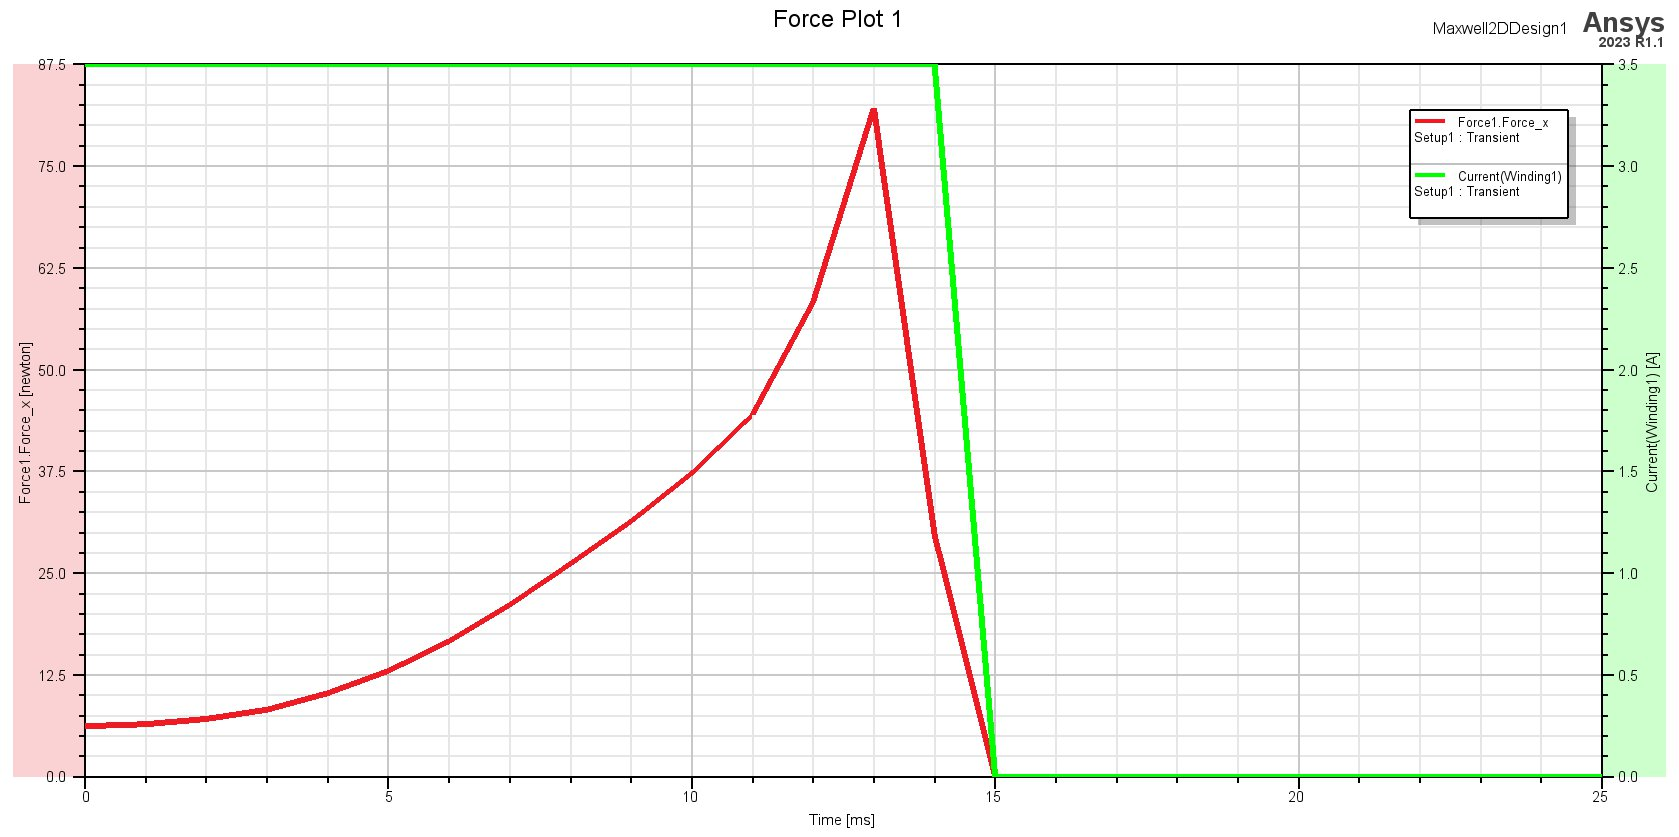
\includegraphics[width=13cm]{FigurasMemoria/S3ForceCurrent.jpg}
    \caption{Fuerza (rojo) y corriente (verde) en función del tiempo de la configuración 3.}
    \label{fig:S3ForceCurrent} %Para referenciar -> \ref{fig:figNum}
\end{figure}
\begin{figure}[H]
    \centering
    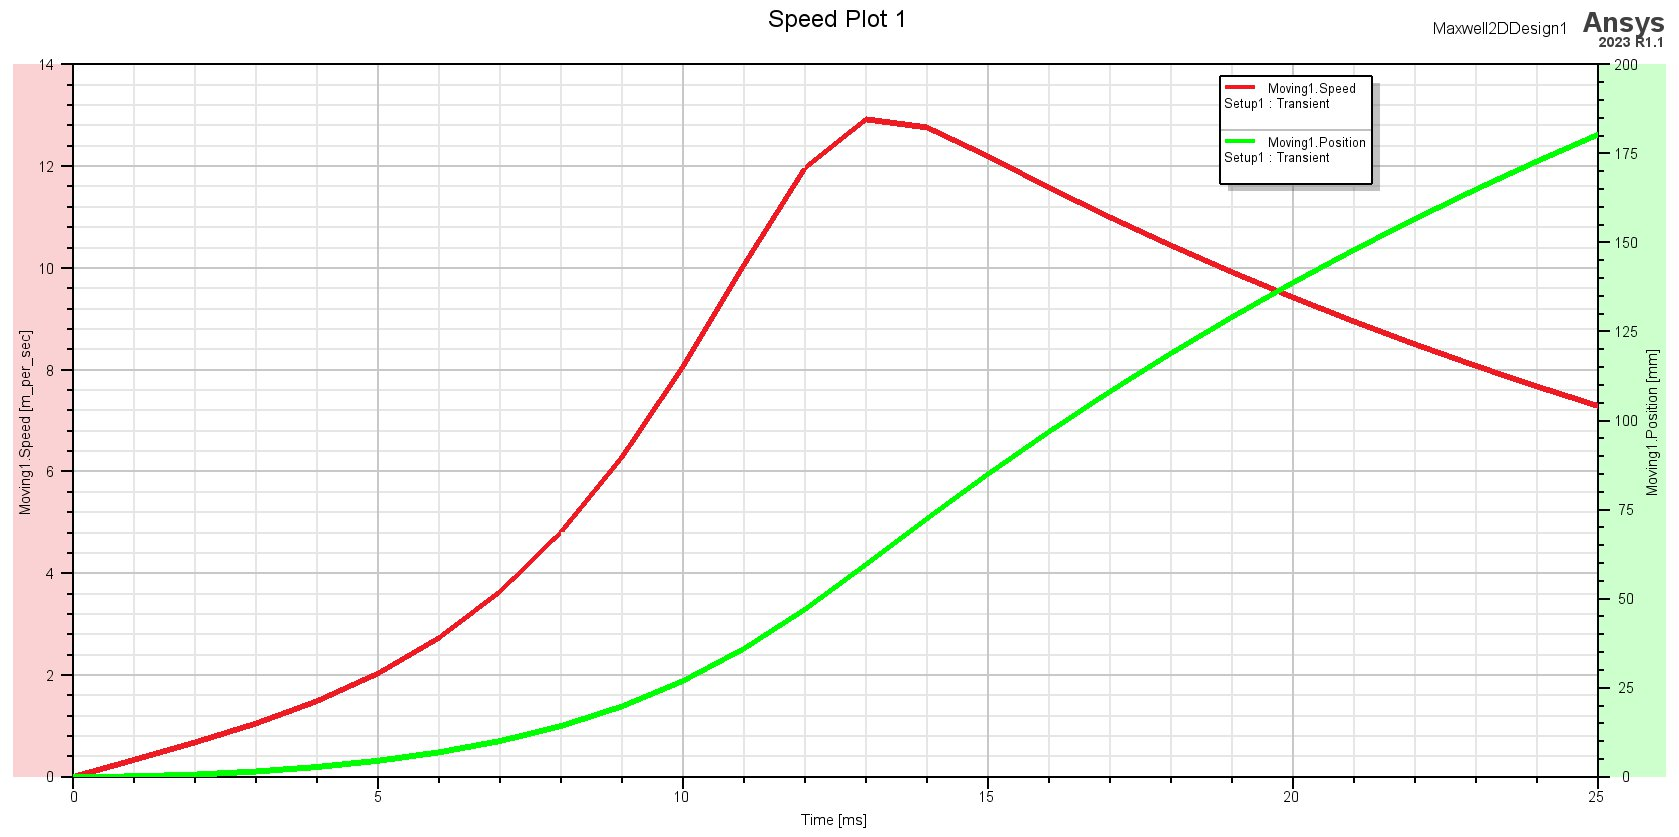
\includegraphics[width=13cm]{FigurasMemoria/S3SpeedPos.jpg}
    \caption{Posición (verde) y velocidad (rojo) en función del tiempo de la configuración 3.}
    \label{fig:S3SpeedPos} %Para referenciar -> \ref{fig:figNum}
\end{figure}

Esta configuración proporciona la evolución de la fuerza según el sistema que queremos crear, dejando de alimentar la bobina antes de que los centros estén alineados y permitiendo que el vástago siga avanzando por inercia, lo cual podemos comprobar observando la gráfica en la figura \ref{fig:S3SpeedPos}, en la que la posición no decrece en ningún momento. Sin embargo, los resultados de la magnitud de la fuerza no son verosímiles, pues son 40 veces mayores (\(F_{max}\approx 80~N\)) a la fuerza obtenida en la prueba de referencia (figura \ref{fig:dinamometro}).

Con esto se dará por finalizado el apartado de simulaciones. Aunque se ha encontrado una configuración que imita correctamente el comportamiento del sistema, los resultados obtenidos no son precisos en términos de magnitud. Dado que no se ha logrado avanzar en la mejora de la precisión de los resultados, se ha decidido no continuar dedicando más tiempo a afinar esta configuración. Se analizará en detalle lo obtenido en el apartado de validación de modelos (\ref{sec:resultados}).

\newpage
\subsection{Prototipo}
\label{subsec:prototipo}

\newpage
\section{Resultados}

\newpage
\section{Discusión y conclusiones}

\newpage
\begin{flushleft}
  \bibliographystyle{abbrvnat}
  \bibliography{referencias}
\end{flushleft}

\newpage
\section*{Anexo I. Código de MATLAB\textsuperscript{\textregistered} para la calculadora de fuerza.}
\label{sec:anexo1}
En este anexo se presenta el código escrito para la calculadora expuesta en el apartado de cálculo analítico (\ref{sec:analitico}). El código para la calculadora es ligeramente diferente ya que recibe las variables del campo \textit{Value} de los componentes de la interfaz en lugar de desde un valor numérico fijo, pero el procedimiento que ejecuta es el mismo que se muestra a continuación:

\begin{lstlisting}[style=Matlab-editor]
    % Propiedades electromagneticas
    mu0 = 4 * pi * 10^-7; % Permeabilidad del vacio [H/m]
    mu_fe = 5000; % Permeabilidad relativa del hierro
    N = 500; % Numero de espiras
    I_c = 3.65; % Corriente de la bobina

    % Geometria
    h_c = 0.05321; % Longitud de la bobina [m]
    r_c = 0.01064; % Radio externo de la bobina [m]
    l_fe = 0.096; % Longitud del vastago [m]
    r_fe = 0.003045; % Radio del vastago [m]

    S_c = pi * r_c ^ 2; % Seccion de la bobina [m^2]
    S_bar = pi * r_fe ^ 2; % Seccion del vastago [m^2]
    S_disp = 2 * S_c; % Seccion de dispersion [m^2]

    % Vectores espaciales
    num_points = 2000; % Numero de puntos
    x = linspace(0, h_c, num_points); % Region de movimiento

    % Definicion de los vectores magneticos
    R_dispc = zeros(size(x));
    R_phi = zeros(size(x));
    R_B = zeros(size(x));
    R_airc = zeros(size(x));
    R_total = zeros(size(x));
    Phi = zeros(size(x));
    B = zeros(size(x));
    F = zeros(size(x));

    % Calculos
    for i = 1:length(x)
        % Calculo de reluctancias:
        R_dispc(i) = h_c / (mu0 * S_disp); % Reluctancia de dispersion de la bobina [H^-1]
        R_B(i) = l_fe / (mu_fe * mu0 * S_bar); % Reluctancia del vastago [H^-1]
        R_phi(i) = ((h_c + l_fe) - x(i)) / (mu0 * S_disp); % Reluctancia de dispersion [H^-1]
        R_airc(i) = (h_c - x(i)) / (mu0 * S_c); % Reluctancia del aire dentro de la bobina [H^-1]

        R_total(i) = R_dispc(i) + R_phi(i) + R_B(i) + R_airc(i); % Reluctancia total [H^-1]
        
        % Flujo [Wb]
        Phi(i) = (N * I_c) / R_total(i);
        
        % Induccion magnetica [T]
        B(i) = Phi(i) / S_bar;

        % Fuerza en x(i) [N]
        F(i) = 0.5 * B(i)^2 * S_bar / mu0;
    end

    % Graficas

    % Reluctancias R[H^-1]
    figure;
    hold on;
    plot(x, R_dispc, 'r', 'DisplayName', 'R_{dispc}');
    plot(x, R_B, 'g', 'DisplayName', 'R_{bar}');
    plot(x, R_phi, 'b', 'DisplayName', 'R_{phi}');
    plot(x, R_airc, 'b', 'DisplayName', 'R_{airc}');
    plot(x, R_total, 'k', 'DisplayName', 'R_{total}');
    xlabel('Posicion del vastago [m]');
    ylabel('Reluctancias [H^-1]');
    title('Reluctancias vs posicion');
    legend show;
    legend('Location', 'best');
    grid on;
    hold off;

    % Induccion magnetica B[T]
    figure;
    plot(x, B, 'LineWidth', 2);
    xlabel('Posicion del vastago [m]');
    ylabel('Induccion magnetica [T]');
    title('Induccion magnetica vs posicion');
    grid on;

    % Fuerza [N]
    figure;
    plot(x, F, 'LineWidth', 2);
    xlabel('Posicion del vastago [m]');
    ylabel('Fuerza magnetica [N]');
    title('Fuerza vs posicion');
    grid on;
\end{lstlisting}

\newpage
\section*{Anexo II. Configuraciones transitorias.}
En este anexo se muestran las diferentes condiciones de inicio de las simulaciones transitorias. 




\end{document}